%% https://towardsdatascience.com/handling-imbalanced-datasets-in-machine-learning-7a0e84220f28

%% https://www.researchgate.net/profile/Kahraman_Kostas/publication/328512658_Anomaly_Detection_in_Networks_Using_Machine_Learning/links/5bd1d1bf458515343d58eddc/Anomaly-Detection-in-Networks-Using-Machine-Learning.pdf

%% http://www.diva-portal.org/smash/get/diva2:1255686/FULLTEXT02.pdf

%% https://ir.lib.uwo.ca/cgi/viewcontent.cgi?article=7635&context=etd

%% http://www.jatit.org/volumes/Vol97No17/4Vol97No17.pdf

%% https://repositorio-aberto.up.pt/bitstream/10216/122764/4/357986.2.pdf

%% http://www.indjst.org/index.php/indjst/article/viewFile/139802/99229

%% https://www.mdpi.com/2076-3417/9/20/4396/pdf

%%
%% Modelo de Dissertação de Mestrado do PGEEC atualizado
%% conforme resolução do PGEEC de 08 de Março de 2019.
%%
%% Utiliza a classe pgeec.cls, versão 4.2 ou superior, atualizada conforme
%% as normas da resolução PGEEC de 08 Março de 2019.
%%
%% Abaixo seguem comentários das versões anteiores (histórico).
%%
%% Romeu Reginatto, junho de 2019.
%%-----------------------------------------------------------
%% Modelo de Dissertação de Mestrado do PGEEC atualizado
%% conforme resolução do PGEEC de 08 de Março de 2019.
%%
%% Utiliza a classe pgeec.cls, versão 4.2, atualizada conforme
%% as normas da resolução PGEEC de 08 Março de 2019.
%%
%% Abaixo seguem comentários das versões anteiores (histórico).
%%
%% Romeu Reginatto, março de 2019.
%% -------------------------------------------------------
%% Modelo de dissertação do PGEEC atualizado em set/2016.
%% Utiliza a classe pgeec.cls, versão atualizada da 
%% classe pgesde.cls de 25 de agosto de 2011.
%%
%% São mantidos todos os comentários do histórico do modelo.
%%
%% Romeu Reginatto, setembro de 2016;
%% -----------------------------------------------------
%%
%% Arquivo modelo para elaboração de dissetações de
%% mestrado do PGESDE. Este modelo segue as resoluções
%% internas do PGESDE que definem as normas técnicas
%% para a apresentação de dissertações de mestrado.
%% 
%% Este modelo foi elaborado por meio de alterações
%% e adequações feitas sobre o modelo disponibilizado
%% na internet por Eleri Cardozo, da Faculdade de
%% Engenharia Elétrica da UNICAMP. Abaixo são mantidos
%% os comentários do modelo original.
%% 
%% Para elaboração deste modelo foi também utilizada
%% a classe sbatex.cls da SBA -- Sociedade Brasileira
%% de Automática, elaborado por Mauricio C. de Oliveira, 
%% mcdeoliveira@ieee.org, 18/12/2000
%%
%% Romeu Reginatto, 25 de agosto de 2011
%% ----------------------------------------------------
%%
%% Arquivo principal para teses de mestrado e doutorado
%% Este modelo de tese foi baseado na tese de doutorado
%% de Luis Fernando Faina (Dez. 2000) e na tese de
%% mestrado de José Cândido Silveira Santos Filho
%% (Agosto de 2003)
%%
%% NOTA: A PUBLICAÇÃO DESTE MODELO VISA APENAS
%% ORIENTAR OS PÓS-GRADUANDOS NA PREPARAÇÃO DE 
%% SUAS TESES. A COMISSÃO DE PÓS-GRADUAÇÃO DA
%% FEEC NÃO PROVÊ ASSISTÊNCIA NO USO DAS
%% FERRAMENTAS NECESSÁRIAS AO USO DESTE MODELO
%% (LATEX, XFIG, ETC.)
%%
%% Eleri Cardozo, Agosto de 2003.
%%

\documentclass[final]{pgeec}
%
% rascunho - imprime capa, sumário e elementos textuais
% banca - gera versão para impressão para a banca
% final - gera versão final impressa 
% digital - gera versão final para publicação digital
%
% Na opção "banca" somente a ficha catalográfica não é impressa. Todos os demais 
% elementos são necessários (afora os que são opcionais e não serão incluídos na 
% versão final).
%
% Para produzir a versão pdf a ser enviada à biblioteca para produzir a ficha catalográfica, utilizar a opção "final".
%
% A versão final é apresentada em 2 formatos: impressa e digital. Ambas devem conter
% a ficha catalográfica e a folha de aprovação assinada.
% - Para a versão impressa (usar opção "final"):
%        1. A folha de aprovação deve ser original. Substituir a folha de aprovação impressa na opção "final" pela folha de aprovação assinada, em cada volume.
%        2. A ficha catalográfica deve ser idêntica à enviada pela biblioteca. Sugere-se efetuar cópia diretamente sobre a folha em branco impressa na opção "final".
%
% - Para a versão digital ("usar opção "digital"):
%        1. A folha de aprovação assinada deve ser escaneada. Recortar do arquivo escaneado aproximadamente o tamanho da margem da folha. Produzir um arquivo .eps que será incluído automaticamente pelo latex na opção "digital".
%        2. A ficha catalográfica deve ser escaneada da versão original impressa ou então convertida do formato pdf para eps. No caso de ser escaneada, recortar aproximadamente o tamanho exato do texto da ficha e converter para o formato eps. O latex fará a importação automática do arquivo eps informado, na opção "digital".
%

%% Comandos para facilitar a edição 
\newcommand{\cpp}{\texttt{C$++$}}
\ifdefined\latex \renewcommand{\latex}{\LaTeX} \else \newcommand{\latex}{\LaTeX} \fi

%% Comandos para utilização de uma nota de rodapé mais de uma vez na mesma página sem duplicação
\makeatletter
\newcommand\footnoteref[1]{\protected@xdef\@thefnmark{\ref{#1}}\@footnotemark}
\makeatother


\begin{document}

%% Identificação do Trabalho
%%
\autor{Gustavo dos Santos Vieira}
\titulo{Construção de Modelos de Detecção de Intrusão baseados em Redes Neurais Artificiais utilizando o \textit{dataset} CICIDS2017}
\ano{2020}


%% Identificacao do orientador e orientador(es) (se houverem)
%
\orientador{Renato Bobsin Machado}
\coorientador{Nome do Coorientador 1}


%% Identificacao da Banca
%
\datadefesa{12/03/2020} 
\bancaorientador{Prof. Dr.}{\NomeOrientador}{Universidade Estadual do Oeste do Paraná}{UNIOESTE}
\bancacoorientador{Prof. Dr.}{Rômulo César Silva}{Universidade Estadual do Oeste do Paraná}{UNIOESTE}
\banca{Prof. Dr.}{Thiago França Naves}{Universidade Tecnológica Federal do Paraná}{UTFPR}
\banca{Prof. Dr.}{Romeu Reginatto}{Universidade Estadual do Oeste do Paraná}{UNIOESTE}


%% Definicao de Elementos Pre-Textuais
%
\ArquivoFicha{PreTextuais/Ficha} % Necessário para a opção "digital"
\ArquivoResumo{PreTextuais/resumo}
\ArquivoAgradecimentos{PreTextuais/agradecimentos}
\dedicatoria{Dedico este trabalho a todos. \\ E a tudo.} % Opcional
%\epigrafe{``Afirmo que a capacidade é inata, \\   mas o conhecimento adquirido.'' \\ John Locke } % Opcional

% Folha de Aprovação Assinada Escaneada para a Versão Digital da Dissertação
% Converter para o eps (ou pdf se usar pdflatex)
%\ArquivoFolhaAprovacao{PreTextuais/FolhaAprovacaoAssinada}  % necessário para a opção "digital"

%% Listas Opcionais
% Descomentar para incluir na dissertação
\IncluiListaFiguras % Inclui Lista de Figuras
\IncluiListaTabelas % Inclui Lista de Tabelas
\IncluiListaSimbolos % Insere Lista de Símbolos construída pelo comando \simbolo
%\ArquivoSimbolos{PreTextuais/simbolos} % Insere Lista de Símbolos do arquivo indicado
\IncluiListaSiglas % Insere Lista de Siglas construída pelos comandos \sigla e \abreviatura
%\ArquivoSiglas{PreTextuais/siglas} % Insere Lista de Siglas do arquivo indicado


\frontmatter
\MakePreTextuais  


%% Elementos Textuais
%
\mainmatter
%%
%% Introdução
%%
\chapter{Introdução}
\label{introducao}

O crescimento tecnológico ocorrido nas últimas décadas constitui fator essencial e decisivo para o desenvolvimento de distintas áreas do conhecimento. O compartilhamento de informações mediante ambientes computacionais tem aumentado de maneira exponencial, visto que a vasta maioria das empresas consolidadas no mercado, independente da área de atuação, utilizam de sistemas de informação e redes de computadores para controle de seus respectivos negócios \cite{machado2005}.

Nesse contexto, onde informações restritas e confidenciais são compartilhadas em redes ao redor do mundo, o número de criminosos digitais (crackers) aumentou fortemente  \cite{nakamura2002}, o que pode ser observado na Figura \ref{fig:cert}. Assim como na sociedade, a segurança é marcada por uma evolução contínua e cíclica. A medida que novas modalidades de crimes são concebidas, em contrapartida, medidas para combater esses crimes são desenvolvidas. Além disso, os novos crimes sempre terão como alvo pontos pouco policiados ou vulnerabilidades do ambiente computacional, no caso do mundo digital \cite{nakamura2002}. Neste contexto, os ataques às redes de computadores, visando a captura de informações privilegiadas, se tornaram comuns e a diversidade dos ataques gerou a necessidade de investimento financeiro e intelectual na segurança de redes de computadores.

\begin{figure}[ht]
    \centering
    \includegraphics[scale=0.5]{Cap1/cert.png}
    \caption{Incidentes de segurança reportados ao CERT. Fonte: www.cert.br}
    \label{fig:cert}
\end{figure}


Dentre os modos mais comuns para a detecção e proteção contra invasões citam-se os Sistemas de Detecção de Intrusão (SDI), os quais atuam auxiliados por mecanismos de monitoramento de redes de computadores, com a finalidade de identificar ações que possam comprometer a integridade, confidencialidade ou disponibilidade de recursos \cite{crosbie1995} e aplicar medidas de correção de violações ocorridas. 

Entre os métodos usados na detecção de intrusão em redes, as estratégias adotadas são diversas, podendo utilizar sistemas especialistas, redes neurais artificiais, mineração de dados, agentes móveis, sistemas imunológicos artificiais (SIA), entre outros \cite{machado2005,delima2005,sujatha2012,hashemi2013,paiva2011}.

A aplicação de técnicas de inteligência artificial voltada à segurança computacional tem sido muito explorada nos últimos anos, com o objetivo de otimizar os métodos convencionais de detecção.

\section{Proposta}

\section{Estrutura do Trabalho}

\begin{comment}

https://www.quora.com/Why-is-it-better-to-use-Softmax-function-than-sigmoid-function


Why Use a One Hot Encoding?

A one hot encoding allows the representation of categorical data to be more expressive.

Many machine learning algorithms cannot work with categorical data directly. The categories must be converted into numbers. This is required for both input and output variables that are categorical.

We could use an integer encoding directly, rescaled where needed. This may work for problems where there is a natural ordinal relationship between the categories, and in turn the integer values, such as labels for temperature ‘cold’, warm’, and ‘hot’.

There may be problems when there is no ordinal relationship and allowing the representation to lean on any such relationship might be damaging to learning to solve the problem. An example might be the labels ‘dog’ and ‘cat’

In these cases, we would like to give the network more expressive power to learn a probability-like number for each possible label value. This can help in both making the problem easier for the network to model. When a one hot encoding is used for the output variable, it may offer a more nuanced set of predictions than a single label.


# SMOTE proposes several variants by identifying specific samples to consider
# during the resampling. The borderline version will detect which point to
# select which are in the border between two classes.

\end{comment} % Incluir aqui os capítulos da dissertação
%%
%% Capítulo 1: Modelo e Descrição Geral para quem usa o LaTeX
%%
\chapter{Fundamentação Teórica}
\label{Cap:fundamentacao}

Neste capítulo tem-se como objetivo apresentar conceitos e fundamentos relacionados as áreas de segurança computacional e inteligência artificial, as quais são de interesse primordial para o presente trabalho.

Na seção de segurança computacional, são citados alguns dos tipos de ameaças existentes, definição e conceitos da linha de pesquisa de detecção de intrusão, assim como os sistemas de detecção de intrusão (SDI) e suas principais características arquiteturais.

A seção de inteligência artificial apresenta contextualização acerca de temas como aprendizado de máquina, aprendizado supervisionado, tipos de modelos e seus paradigmas, tal como métricas geralmente utilizadas para avaliação dos modelos construídos.

\section{Segurança Computacional}
\label{Sec:seguranca-computacional}
A exposição de grande volume de informação em uma velocidade, até poucos anos atrás, inimaginável é uma consequência da popularidade de Internet e da facilidade de acesso à mesma, após a chegada de dispositivos móveis, computadores pessoais, televisores inteligentes, entre outros.

De mesmo modo que este fenômeno foi responsável por vários avanços tecnológicos benéficos a sociedade, foi também responsável pelo crescimento drástico de ocorrências de atividades ilícitas no mundo digital, visto que todo sistema de informação ou infraestrutura computacional pode estar sujeito a apresentar vulnerabilidades.

Para identificar e auxiliar em medidas a serem tomadas, diante do acontecimento de eventos maliciosos em ambiente computacional, a área de pesquisa denominada ``Segurança Computacional`` foi criada e está em constante aprimoramento por meio de pesquisas científicas. Embora a amplitude de temas abordados dentro da área de segurança seja enorme, \citeasnoun{gollmann2010} divide a mesma em quatro partes, de acordo com diferentes interesses:

\begin{itemize}
    \item Controle de acesso a um sistema;
    \item Controle de acesso a recursos gerenciados por um sistema;
    \item Proteção de dados transmitidos entre sistemas;
    \item Proteção de sistemas contra \textit{inputs} maliciosos.
\end{itemize}

Cada um dos tópicos citados e discutidos por \citeasnoun{gollmann2010} tem suma importância no que se refere a segurança computacional, pois englobam praticamente todos os focos de incidentes no mundo digital. O presente trabalho, por sua vez, encontra-se enquadrado no tópico de "proteção de dados sendo transmitidos entre sistemas", visto que são levados em conta principalmente eventos ocorridos durante a comunicação de computadores por meio de redes de computadores, ou seja, mediante análise de tráfego de dados.

\begin{comment}
\subsection{Tipos de Ameaças}
\label{Sec:subsecoes}

Tipos de ataques interessantes de abordar:
DoS (Comentar que podem ser utilizadas várias ferramentas: HULK, GoldenEye, Slowloris)
Brute Force (Citando Patator, que oferece suporte pra vários serviços, mas focar em SSH e FTP que estão presentes na CICIDS2017)
PortScan
Botnet
Infiltration (iciss20140_submission_35.pdf downloads)

\end{comment}

\subsection{Detecção de Intrusão}
\label{Sec:figuras}

Eventos intrusivos correspondem àqueles que infringem princípios básicos da segurança computacional, como confidencialidade, integridade, autenticidade e/ou disponibilidade de informações ou recursos. Diante da necessidade e da importância de identificar e analisar esses eventos, delineou-se a área de detecção de intrusão, a qual trata-se da linha de pesquisa responsável pelo desenvolvimento de técnicas que objetivam a identificação de intrusões e atividades maliciosas, a fim de alertar e possibilitar contramedidas aos incidentes ocorridos.

SDI são considerados uma das principais ferramentas utilizadas para esta tarefa, visto que são capazes de combinar diferentes estratégias e características arquiteturais, com o intuito de  identificar comportamentos anômalos que apontem suspeitas de que atividades não lícitas estejam sendo desempenhadas em computadores, sistemas, redes de computadores, entre outros.

Embora diversas classificações de sistemas de detecção de intrusão tenham sido propostas ao longo do tempo, não existe uma taxonomia aceita de forma padronizada e universal, visto que as abordagens possuem prós e contras, acarretando em \textit{tradeoffs} que devem ser avaliados de acordo com o objetivo específico do sistema de detecção de intrusão em questão. Alguns desses aspectos são apresentados a seguir \cite{lazarevic2005}:

\begin{itemize}
    \item \textbf{Fonte de dados:} alguns exempos de fonde dados de SDI são \textit{host} (sistema operacional da máquina local), rede de computadores, logs de aplicações, sensores de alertas.
    \item \textbf{Estratégia de análise:} análise por abuso compreende na técnica mais comumente utilizada, onde o SDI monitora os dados a fim de identificar a ocorrência de comportamentos previamente catalogados, enquanto na análise por anomalia o SDI busca por comportamentos que diferem de atividades definidas e consideradas normais, utilizando diferentes técnicas como regras, métodos estatísticos, cálculo de distâncias, definição de perfis, e outros. Vários SDI também utilizam abordagens híbridas.
    \item \textbf{Frequência de uso:} a análise pode ser realizada tanto em tempo real, monitorando fluxo contínuo de dados, quanto periodicamente, de forma \textit{offline}, investigando lotes de dados, como em auditorias, por exemplo.
    \item \textbf{Arquitetura:} quanto a arquitetura, os SDI podem ser centralizados ou distribuídos. Os SDI centralizados são geralmente utilizados para detectar intrusões feitas em um único sistema a ser monitorado. Com o surgimento de ataques coordenados e distribuídos, com várias máquinas envolvidas, surgiu a necessidade de também monitorar sistemas de forma distribuídas e cooperativa.
    \item \textbf{Tipo de resposta:} SDI podem agir de forma ativa (aplicando contramedidas, como alteração nos serviços disponíveis em um servidor, por exemplo) ou passiva (apenas registrando o comportamento ilícito, eventualmente emitindo alertas) quando uma atividade anômala é identificada.
\end{itemize}

Ainda que não haja consenso na definição de características dos SDI, de modo geral, todos seguem uma estrutura bastante semelhante uns aos outros no que se refere a seus componentes. Na Figura \ref{fig:ids-components} é apresentado um \textit{framework} arquitetural que ilustra os principais componentes que compõem um sistema de detecção de intrusão:

\begin{figure}[!hbt]
\centering \includegraphics[width=12cm]{{Cap2/ids-components-framework.png}}
\caption{Arquitetura básica de componentes de sistemas de detecção de intrusão (SDI). \cite{lazarevic2005}}
\label{fig:ids-components}
\end{figure}

Conforme apresentado na Figura \ref{fig:ids-components}, os principais componentes são os seguintes:

\begin{itemize}
    \item \textbf{Coletor de dados (\textit{Data gathering device})}: responsável pela coleta de dados do sistema monitorado, mediante geração de \textit{log} e/ou captura e processamento de pacotes de dados, por exemplo.
    \item \textbf{Motor de análise de detecção intrusão (\textit{Detector - Intrusion detection analysis engine}}): componente que processa as informações coletadas para identificar atividades intrusivas.
    \item \textbf{Base de conhecimento (\textit{Knowledge base})}: geralmente contém os dados capturados pelos sensores de coleta, porém de maneira formatada e pré-processada, de modo a serem utilizados pelo motor de análise.
    \item \textbf{Dispositivo de configuração (\textit{Configuration device})}: provê informações sobre o estado atual do SDI.
    \item \textbf{Componente de resposta (\textit{Response component})}: componente que possui a responsabilidade de aplicar contramedidas quando uma intrusão é detectada, podendo ser automático ou necessitar de intervenção humana.
\end{itemize}

Neste contexto, este trabalho encontra-se concentrado no desenvolvimento de técnicas que objetivam melhorias nos resultados apresentados pelo motor de análise de detecção de intrusão, mediante processamento de informações disponíveis em uma base de conhecimento. Neste caso, a base de conhecimento corresponde a base de dados CICIDS 2017, a qual é descrita na seção \ref{Subsec:cicids2017} (página \pageref{Subsec:cicids2017}). 

\section{Inteligência Artificial}
\sigla{IA}{Inteligência Artificial}
\sigla{AM}{Aprendizado de Máquina}
\sigla{MD}{Mineração de Dados}
\sigla{KDD}{\textit{Knowledge Discovery in Databases}}

O tema Inteligência Artificial (IA) possui diversas definições, as quais  geralmente remetem a área do conhecimento que busca reproduzir capacidades humanas como pensamentos, razão, percepções subjetivas, ou somente, inteligência. \citeasnoun{winston1992} define IA como "o estudo das computações que tornam possível perceber, raciocinar, e agir", enquanto \citeasnoun{rich1991} refere-se a este domínio como "o estudo que visa permitir computadores fazerem coisas que, até o momento, pessoas fazem melhor".

Devido a imensa subjetividade das questões que envolvem o estudo de IA, a tarefa de mensurar o quão inteligente um computador pode ser torna-se algo bastante complexo de ser feito. Desse modo, em 1950, Alan Turing propôs um teste que fornece uma definição operacional para "inteligência". Segundo \citeasnoun{turing1950}, um computador é considerado inteligente quando uma pessoa, após fornecer perguntas escritas, não souber determinar se as respostas foram fornecidas por um computador ou outra pessoa.

Por sua vez, \citeasnoun{russell2009} ressalta a dificuldade de programar um computador capaz de passar em um teste deste gênero. Além disso, \citeasnoun{russell2009} também defende que este feito requer que o computador possua capacidade de processamento de linguagem natural, armazenamento de uma representação do conhecimento que possui, tal como devem existir mecanismos de raciocínio automatizado e aprendizado de máquina. Dessa forma, o computador seria capaz de comunicar-se em linguagem natural, como, por exemplo, em inglês, reter conhecimento, utilizar o conhecimento armazenado a fim de responder questões e chegar a conclusões próprias, além de adaptar-se e extrapolar padrões.

\subsection{\textit{Knowledge Discovery in Databases} (KDD)}

Diante da imensidão de dados sendo gerados cotidianamente, pelos inumeráveis dispositivos conectados à Internet, a necessidade do desenvolvimento de técnicas e estudos que possibilitem a extração de conhecimento desses dados cresce também de forma expressiva. A análise de dados, em busca de padrões que permitam a extração de informações de um conjunto de dados, é uma tarefa realizada há séculos, mesmo que com técnicas pouco avançadas, ou até mesmo, manualmente. O avanço da computação, vide o crescimento exponencial da capacidade de captura, armazenamento e processamento de dados, é responsável também pelo grande aumento da complexidade dos dados a serem analisados, tornando inviável a análise manual. 

A descoberta de conhecimento em bases de dados (do inglês, \textit{"knowledge discovery in databases"}), também conhecida como Mineração de Dados (MD), visa solucionar problemas por meio da análise de dados que já estão armazenados e, de alguma forma, organizados em ambiente computacional. O KDD é definido como "o processo de descoberta de padrões relevantes em dados" \cite{witten2005}. Também é possível referir-se a MD como a área que está interessada em desenvolver técnicas para descobrir e descrever padrões em dados, ou então, como uma ferramenta que auxilia o entendimento desses dados e a realização de predições a partir da análise dos mesmos.

O processo de mineração de dados está dividido em algumas etapas essenciais, as quais são muitas vezes desempenhadas, de forma iterativa com objetivo de refinar ideias e entendimentos da área de aplicação, tal como do comportamento dos algoritmos e as estratégias escolhidas quando aplicadas aos diferentes tipos de dados existentes. Embora ajam opiniões divergentes acerca das fases que compõem o processo de MD, a seguir são apresentadas as etapas consideradas básicas \cite{kantardzic2011, kurgan2006}:

\begin{itemize}
    \item \textbf{Definição do problema:} visto que a maioria dos problemas que busca-se solucionar mediante MD são de um domínio muito específico, é imprescindível a dedicação de bastante esforço na definição do problema, onde o ideal é que duas figuras estejam presentes: um especialista em mineração de dados e um especialista na área de aplicação.
    
    \item \textbf{Coleta de dados:} a captura dos dados a serem minerados pode ser realizada de dois (2) modos gerais (com experimento modelado ou por meio da abordagem observacional). Na primeira abordagem, o especialista encarregado pela geração dos dados possui total controle do processo, enquanto na segunda estratégia são capturados dados aleatórios e com distribuições muitas vezes desconhecidas, a qual representa o comportamento da maioria das áreas que lidam com informações do mundo real.
    
    \item \textbf{Pré-processamento:} nesta etapa, os dados geralmente estão disponibilizados em conjuntos, representados e organizados em meio digital. Alguns modos clássicos de armazenamento são bancos de dados, planilhas e tabelas de representação atributo-valor. Embora já organizados de algum modo que possibilite o processamento das informações, algumas tarefas são necessárias para que as próximas etapas do processo sejam possíveis, como limpeza dos dados, tratamento de \textit{outliers}, duplicatas e dados faltantes, seleção de atributos, normalização dos dados, entre outras.
    
    \item \textbf{Mineração:} a principal tarefa desempenhada nesta fase é a aplicação de técnicas e algoritmos capazes de, de modo automático ou semiautomático, identificar padrões e gerar uma estrutura que represente o conhecimento implícito nos dados. As abordagens, algoritmos e parâmetros dos algoritmos utilizados nessa fase podem variar dependendo de diversos aspectos, como, por exemplo, a natureza e características do conjunto de dados, ou então que tipo de análise pretende-se realizar com o modelo gerado. De acordo com os objetivos do presente trabalho, nas seções seguintes serão abordados com mais detalhes outros aspectos levados em conta na fase de mineração do processo de MD.
    
    \item \textbf{Interpretação/Avaliação:} solucionar problemas complexos geralmente requer a construção de modelos complexos, os quais na maioria dos casos são responsáveis por auxiliar em tarefas de tomada de decisão. Por comumente serem empregados em tarefas importantes e críticas, a avaliação dos modelos resultantes do processo de MD compreende uma das fases mais relevantes do processo como um todo, onde são utilizadas diversas métricas e métodos analíticos para mensurar a capacidade de generalização do problema por parte do modelo construído.
\end{itemize}

\subsection{Aprendizado de Máquina}
\label{Sec:aprendizado}

A fim de entender o conceito de Aprendizado de Máquina (AM), diversas questões filosóficas podem ser levantadas em torno do que de fato se entende por "aprendizado" e como seria possível performar e mensurar o aprendizado de um computador \citeasnoun{witten2005}. Conforme mencionado no trabalho desenvolvido por \citeasnoun{russell2009}, AM é um dos principais fatores necessários para que um computador possa ser considerado inteligente, visto que trata-se da subárea da IA responsável pelo desenvolvimento de algoritmos e construção de sistemas com capacidade de aquisição de conhecimento de maneira automatizada.

O aprendizado ocorre por parte de um programa de computador quando o mesmo realiza determinada tarefa \textit{T}, e é capaz de melhorar sua performance em \textit{T}, medida por \textit{P}, a partir de experiências \textit{E} observadas ou vivenciadas \cite{mitchell1997}. A capacidade de reconhecimento de palavras ditas, veículos autônomos ou identificação automática de objetos em imagens são alguns exemplos de tarefas que computadores podem aprender a desempenhar.

Diante do desafio de extrair conhecimento de dados brutos, diversos métodos surgiram ao longo do desenvolvimento da subárea de AM, sendo que uma das estratégias mais utilizadas é o aprendizado indutivo. A inferência indutiva, como também pode-se referir ao aprendizado indutivo, compreende a concepção de que é possível obter conclusões generalistas a partir de fatos observados, ou seja, a generalização do problema é dada a partir de um conjunto suficientemente grande de registros de eventos de interesse \cite{kantardzic2011}. Vale ressaltar a extrema valia da relevância e da representatividade dos dados, pois dados insuficientes ou pouco descritivos podem levar a conclusões errôneas. Esta técnica é empregada em vários dos problemas englobados pela subárea de AM, como regressão, clusterização (ou agrupamento), classificação, e outros.

Métodos de aprendizado indutivo estão categorizados em diferentes tipos: supervisionado, não supervisionado, semi-supervisionado e reforço. A Figura \ref{fig:tipos-aprendizado} ilustra os diferentes tipos de aprendizado.

\begin{figure}[H]
\centering \includegraphics[width=1.0\textwidth]{{Cap2/tipos-aprendizado.png}}
\caption{Hierarquia dos tipos de aprendizado.}
\fonte{Fonte: \citeasnoun{lazarevic2005}}
\label{fig:tipos-aprendizado}
\end{figure}

No aprendizado supervisionado é necessário que os dados estejam rotulados, ou seja, apresentam qual o \textit{output} esperado pelo algoritmo. O \textit{output} é comumente chamado de rótulo ou classe. Desse modo, é possível definir um subconjunto de treinamento a ser utilizado para aquisição de conhecimento, enquanto outro subconjunto de testes é utilizado para cálculo de métricas de avaliação do modelo, como a acurácia, por exemplo. Quando os possíveis rótulos são valores finitos, o problema de aprendizado é chamado de classificação, podendo ser binária (dois possíveis valores), multi-classe (mais de dois valores possíveis) ou multi-rótulo (onde, independentemente do número de possíveis valores, existe a possibilidade de um único exemplo pertencer a mais de uma classe). Quando as possíveis classes existentes são valores contínuos, chama-se de regressão o problema de aprendizado.

O aprendizado não supervisionado, por sua vez, ocorre quando não há a presença dos rótulos, e é necessário que os algoritmos empregados no aprendizado sejam capazes de agrupar os exemplos contidos na base de dados somente analisando as características dos mesmos. Existe ainda o chamado semi-supervisionado, onde apenas parte das classes dos exemplos existentes são fornecidas. Dessa forma, os algoritmos tem o objetivo de buscar formas de, baseado nas observações com rótulo conhecido, aumentar o tamanho do conjunto rotulado, muitas vezes a fim de viabilizar o aprendizado supervisionado. Por fim, no aprendizado por reforço, o conhecimento é obtido por meio do resultado de decisões feitas pelo próprio sistema em processo de aprendizagem seguinte a estratégia de tentativa e erro. O resultado das decisões tomadas pode ocasionar recompensas boas ou ruins, e essa é a métrica utilizada para dimensionar o sucesso ou não da ação desempenhada pelo sistema.

O presente trabalho aborda a detecção de eventos intrusos e anômalos em ambiente computacional como um problema de classificação, manipulando a base de dados, de modo que possam ser avaliados dois cenários distintos: classificação binária e classificação multi-classe.

\subsection{Paradigmas}
\label{Sec:paradigmas}

As diversas abordagens e estratégias desenvolvidas ao longo dos anos na área de IA, mais especificamente na subárea de AM, podem ser classificadas de acordo com os paradigmas utilizados pelos algoritmos que as implementam. A seguir são apresentados alguns dos principais paradigmas aplicados em problemas de AM.

\subsubsection{Simbólico}

O paradigma simbólico, seguindo a ideia transmitida pela etimologia da palavra, remete a "sinais", "símbolos", "significados", e afins. Modelos construídos por meio de algoritmos que seguem este paradigma geralmente encontram-se representados na forma de expressões lógicas, árvores de decisão, regras ou redes semânticas \cite{maletzke2009}. Essas estruturas de modelos permitem a análise das regras inferidas nas etapas de treinamento, de modo que um especialista no domínio possa validar o aprendizado ocorrido.

\subsubsection{\textit{Instance-Based}}

Métodos deste gênero como, por exemplo, o algoritmo dos \emph{k} vizinhos mais próximos (K-\textit{Nearest Neighbors}), mantém o conjunto de exemplos de treinamento em memória, ao invés de criar um modelos que os represente. Deste modo, ao classificar um novo exemplo, métricas de distância ou similaridade são calculadas de modo a determinar quais observações, dentre as existentes na base de treinamento, possuem mais semelhanças com o novo elemento a ser classificado \cite{mitchell1997}. Embora ajam diversas vantagens em abordagens dessa natureza, a tarefa de classificação pode ser bastante custosa em comparação a outros mecanismos de classificação.

Poderia


\subsubsection{Genético}

Este paradigma está basicamente pautado na evolução simulada em ambiente computacional, com técnicas embasadas na definição de evolução da área de biologia. Algoritmos genéticos geralmente descrevem as hipóteses como sequências de \textit{bits}, e a interpretação dessas representações variam de acordo com o domínio de aplicação \cite{mitchell1997}. Desta forma, são definidas populações de exemplos iniciais, os quais são modificados de modo iterativo ao longo do que são as chamadas "gerações", mediante operações como reprodução ou mutação, dentre outras. A comparação entre indivíduos de diferentes populações é dada por uma função \textit{fitness}, a qual define uma métrica capaz de elencar os indivíduos mais bem adaptados.

\subsubsection{Conexionista}

O conexionismo, ou paradigma conexionista, é a área que estuda estruturas conhecidas como redes neurais artificiais. Essas estruturas também possuem inspiração biológica e buscam construir modelos mediante a extração de conhecimento implícito, contido nas relações existentes entre \textit{input} e \textit{output} \cite{rajagopalan1993}. Redes neurais artificiais serão abordadas com mais detalhes na seção seguinte.

\section{Redes Neurais Artificiais}

É estimado que o cérebro humano possua aproximadamente 10\textsuperscript{11} neurônios \cite{mitchell1997}, os quais tratam-se de células nervosas capazes de receber, processar e enviar informações. Os bilhares de neurônios também são capazes de conectar-se uns aos outros, possibilitando a construção do que é conhecido por rede neural. É através dessa complexa estrutura que os pulsos elétricos gerados por estímulos, externos ou do próprio corpo humano, são transmitidos e interpretados, possibilitando ao ser humano desempenhar tarefas complexas, como a tomada de decisão. \citeasnoun{haykin2001} define o cérebro como "um computador (sistema de processamento de informação) altamente complexo, não linear e paralelo".

Segundo o mesmo autor, uma das principais motivações para o desenvolvimento da área de redes neurais artificiais é a busca pela adaptação do uso de computadores convencionais, a fim de possibilitar aos mesmos desempenhar tarefas complexas, como reconhecimento de padrões e processamento visual. Por definição, uma rede neural artificial é "uma máquina projetada para modelar a maneira como o cérebro realiza uma tarefa particular ou função de interesse" \cite{haykin2001}.

A Figura \ref{fig:neuronio-biologico} apresenta a estrutura biológica dos neurônios, a qual é formada por corpo celular, dendritos, axônio e terminações do axônio, sendo que cada um possui papel fundamental no processo de recebimento de sinais elétricos e propagação dos mesmos ao longo de todo conglomerado de conexões neurais. A transmissão dos estímulos entre neurônios é denominada sinapse, e pode ser tanto excitatória, quanto inibitória aos chamados neurônios pós-sinápticos \cite{lent2004}.

\begin{figure}[H]
\centering \includegraphics[width=\textwidth]{{Cap2/neuronio-biologico.png}}
\caption{Estrutura de um neurônio biológico.}
\fonte{Fonte: Adaptado de \citeasnoun{poel2019}.}
\label{fig:neuronio-biologico}
\end{figure}

Diante do exposto, para a construção de redes neurais artificiais são necessárias abstrações computacionais dos elementos que compõem a comunicação entre os neurônios, capazes de aprender mediante as interações ocorridas entre si, assim como acontece no cérebro humano. Na Figura \ref{fig:neuronio-artificial}, observa-se uma representação simplificada dessas abstrações. Alguns dos aspectos referentes a essa estrutura, que é comumente chamada de ``neurônio artificial``, serão abordadas nas seções seguintes.

\begin{figure}[H]
\centering \includegraphics[width=\textwidth]{{Cap2/neuronio-artificial.png}}
\caption{Modelo matemático que representa um neurônio artificial.}
\fonte{Fonte: Adaptado de \citeasnoun{haykin2001}}
\label{fig:neuronio-artificial}
\end{figure}

\subsection{Funções de ativação}
\label{subsec:funcoes-ativacao}
Dentre os componentes do modelo matemático que representa o neurônio artificial cita-se a função da ativação. Cada um dos neurônios que compõem uma rede neural é capaz de guardar seu próprio estado interno, e o que determina esse estado é a função de ativação aplicada aos sinais de entrada, após multiplicados pelos ``pesos sinápticos`` e processados pelo ``somador``, conforme apresentado na Figura \ref{fig:neuronio-artificial}. O valor de saída da função de ativação de cada neurônio é então transmitido aos neurônios da próxima camada da rede que possuem conexão com o neurônio em questão.

Funções de ativação devem ser computacionalmente eficientes, dado que, dependendo da arquitetura da rede neural, as mesmas podem ser recalculadas milhões de vezes ao longo do treinamento do modelo neural. Diante disso, diferentes tipos de função de ativação foram propostos ao longo do tempo, geralmente tratando-se de funções matemáticas pouco complexas. Funções de ativação podem ser lineares ou não lineares, sendo que essas primeiras não possibilitam a aplicação do algoritmo \textit{backpropagation}, técnica amplamente utilizada no treinamento de redes neurais para estimar as derivadas necessárias para a definição dos gradientes no treinamento da RNA, possibilitando o ajuste dos pesos dos neurônios a fim de minimizar a perda de informação \cite{hecht1992}.

As funções de ativações não lineares de uso mais comum são apresentadas a seguir \cite{goodfellow2016}:
\begin{enumerate}
    \item \textbf{Sigmoide/Logística:} trata-se de uma função de ativação amplamente utilizada, pois apresenta comportamento balanceado entre linearidade e não-linearidade. Entretanto, características referentes às suas derivativas fazem com que atualmente seja desencorajado o uso das mesmas, com exceção de camadas de saída (para variáveis binárias) e casos específicos de redes recorrentes ou modelos probabilísticos, por exemplo \cite{goodfellow2016}. A saída dessa função é um valor contido no intervalo contínuo de 0 a 1. A função sigmoide é apresentada na Equação \ref{eq:sigmoide}. Na Figura \ref{fig:sigmoide} é possível observar o comportamento da função, tal como a sua derivada.
    \begin{equation}
    \label{eq:sigmoide}
        \sigma (x) ={1 \over 1 + e^{-x}}
    \end{equation}
    
    \begin{figure}[H]
        \centering \includegraphics[width=0.90\textwidth]{{Cap2/sigmoide.png}}
        \caption{Gráfico da função de ativação Sigmoide.}
        \fonte{Fonte: \cite{facure2017}}
        \label{fig:sigmoide}
    \end{figure}
    
    \item \textbf{Tangente Hiperbólica (TanH):} bastante semelhante a função logística, porém com seu valor variando de -1 a 1, fazendo com que a parábola esteja centralizada no 0. A Equação \ref{eq:tanh} exibe a fórmula de cálculo da tangente hiperbólica. Na Figura \ref{fig:tanh}, que apresenta de forma gráfica o comportamento da função e de sua derivativa, é possível observar que o valor da derivada é maior quando comparada a função logística. Diante disso, quando é necessário o uso de uma função sigmoidal, geralmente utiliza-se a função \textit{tanh} \cite{goodfellow2016}.
    \begin{equation}
    \label{eq:tanh}
        tanh(x) = {2\sigma (2x) - 1}
    \end{equation}
    
    \begin{figure}[H]
        \centering \includegraphics[width=0.90\textwidth]{{Cap2/tanh.png}}
        \caption{Gráfico da função de ativação Tangente Hiperbólica.}
        \fonte{Fonte: \cite{facure2017}}
        \label{fig:tanh}
    \end{figure}
    
    \item \textbf{Unidade Linear Retificada (ReLU):} conforme observado na Equação \ref{eq:relu}, trata-se de uma função praticamente linear, com exceção de metade do seu domínio (parte negativa), onde o valor de saída atribuído é zero. Desse modo, as derivativas mantém-se grandes (1, para valores positivos) e constantes, sendo possível também definir como 0 a derivada para valores negativos. Essa característica pode ser observada na Figura \ref{fig:relu}. Essa função de ativação demonstra ser extremamente poderosa diante da simplicidade unida a não linearidade.
    \begin{equation}
    \label{eq:relu}
        ReLU(x) = {max\{0,x\}}
    \end{equation}
    
    \begin{figure}[H]
        \centering \includegraphics[width=0.90\textwidth]{{Cap2/relu.png}}
        \caption{Gráfico da função de ativação Unidade Linear Retificada.}
        \fonte{Fonte: \cite{facure2017}}
        \label{fig:relu}
    \end{figure}
    
    \item \textbf{Softmax:} outro tipo de função de ativação, geralmente utilizada na camada de saída, mas que também pode ser aplicada em camadas ocultas em casos específicos. Funções \textit{softmax} representam uma distribuição probabilística de uma variável discreta, apresentando uma probabilidade para cada valor possível \cite{goodfellow2016}. Ao contrário de funções sigmoide, a \textit{softmax} é capaz de trabalhar com problemas com mais de duas classes.

\end{enumerate}

\subsection{Treinamento}
\label{subsec:treinamento}
Conforme apresentado na Seção \ref{Sec:aprendizado}, existem diferentes paradigmas de aprendizado aplicados na construção de modelos de aprendizado de máquina. RNA realiza o aprendizado mediante um processo iterativo, onde os pesos sinápticos são reajustados, e isso é definido como a tarefa de treinamento da rede \cite{haykin2001}.

O processo de treinamento de RNA, como já mencionado, é realizado através da manipulação dos pesos atribuídos a cada um dos neurônios de entrada. Quando o treinamento é iniciado, esses pesos geralmente são inicializados de forma aleatória, fato que pode resultar em uma rede de baixa performance num primeiro momento, mas que pode convergir para uma rede com alta acurácia ao longos da iterações. Essas iterações são chamadas de épocas. A cada época de treinamento, os pesos são reajustados e então é realizado o treinamento novamente.

Diante disso, utiliza-se de uma função de perda para dar suporte ao reajuste dos pesos sinápticos. A função de perda, por sua vez, é uma das possíveis métricas que visam mensurar a performance de uma rede, onde redes com perda baixa apresentam resultados melhores do que aquelas que possuem perda alta. No aprendizado supervisionado, a perda é comumente calculada com base no erro do modelo, ou seja, a diferença entre os valores preditos e os valores reais dos exemplos da base de treino. Neste contexto, a tarefa de treinamento remete a um problema de otimização, no qual objetiva-se a minimização da perda da RNA.

Diferentes algoritmos de otimização foram propostos e empregados no treinamento de redes neurais ao longo do desenvolvimento da área de aprendizado de máquina. Um dos algoritmos mais simples é o \textit{Stochastic Gradient Descent} (SGD), o qual utiliza de gradientes, que por sua vez são vetores de derivativas, a fim de determinar se o ajuste de pesos da época atual deverá ser feito na direção positiva ou negativa, em busca do cenário ideal onde a perda é zero (0). Uma das limitações desse algoritmo é que um de seus parâmetros, a taxa de aprendizagem, é imutável ao longo do treinamento.

Para contornar esta limitação, outros algoritmos de otimização foram propostos como RMSProp (\textit{Root Mean Square Propagation}) e Adam (\textit{Adaptive Moment Estimation}). Ambos viabilizam uma taxa de aprendizagem dinâmica ao longo do treinamento da rede, embora o algoritmo Adam seja uma melhoria do RMSProp, e por isso têm sido mais utilizado em relação a outros algoritmos de otimização.

Desse modo, o treinamento de uma RNA se dá por meio da utilização de um algoritmo de otimização que busca minimizar a perda existente no modelo neural, sendo que a função de perda compreende em uma métrica para avaliar a performance da rede. O número de épocas pode ser previamente determinado de forma fixa, ou então depender de alguma condição definida na implementação da rede considerando o comportamento de alguns dos parâmetros da mesma, como, por exemplo, um critério de parada baseado em um limiar de perda ou de acurácia do modelo.

\subsection{Arquiteturas}
Outro aspecto essencial na definição de uma RNA é sua arquitetura, o que geralmente remete a sua estrutura, quantidade de neurônios e como os mesmos estão organizados e conectados \cite{goodfellow2016}. A maioria das RNA estão organizadas em sequenciais agrupamentos de neurônios (ou nós), chamados de camadas. Camadas de RNA podem ser de entrada, de saída ou ocultas. Os tipos básicos de camadas podem ser observados na Figura \ref{fig:arquitetura-basica}, onde a camada mais à esquerda corresponde a camada de entrada, a mais à direita corresponde a camada de saída, enquanto as demais são chamadas de camadas ocultas. Vale ressaltar que RNA podem possuir uma ou mais camadas ocultas, enquanto camadas de entrada e saída são únicas.

\begin{figure}[H]
        \centering \includegraphics[width=\textwidth]{{Cap2/arquitetura-basica.png}}
        \caption{Arquitetura simplificada de uma rede neural com duas camadas ocultas.}
        \fonte{Fonte: Adaptado de \citeasnoun{datascienceacademy2019}.}
        \label{fig:arquitetura-basica}
    \end{figure}

A arquitetura disposta na Figura \ref{fig:arquitetura-basica} representa uma estrutura básica que a maioria das RNA seguem, embora possa haver diversas variações no \textit{design} das camadas ocultas, tanto em termos do número de camadas ocultas, quanto em relação ao número de neurônios existentes em cada uma dessas camadas. O \textit{design} dessas camadas intermediárias, ou ocultas, é ponto crucial na definição de um rede neural, principalmente de redes profundas, com mais de uma camada oculta. A área de que estuda redes mais profundas é denominada \textit{Deep Learning}.

No contexto deste trabalho serão abordadas redes nas quais as saídas das camadas são providas como entrada para as camadas posteriores \cite{haykin2001}. Tratam-se das chamadas redes neurais \textit{feedforward}. 
Dentre os diferentes tipos de redes \textit{feedforward}, a \textit{Multilayer Perceptron} (MLP) ganhou popularidade ao longo dos anos devido a sua capacidade de generalizar problemas não linearmente separáveis, o que é o caso de grande parte dos problemas reais existentes \cite{engelbrecht2007}.

Desse modo, com auxílio do algoritmo \textit{backpropagation} apresentado anteriormente, o treinamento se dá mediante propagação dos pesos sinápticos da camada de entrada para a camada de saída, passando por cada uma das camadas ocultas, sendo que nesse momento os pesos mantém-se inalterados. Após, com base no erro calculado utilizando-se do resultado esperado (aprendizado supervisionado) e do valor de saída da última camada, os pesos são ajustados e realiza-se uma nova iteração do treinamento. Considera-se que o treinamento foi concluído quando o erro for suficientemente pequeno. A partir disso, a rede passa a operar apenas em sentido \textit{forward} para a classificação de novos exemplos.

\subsection{Avaliação de Modelos}
\label{Sec:avaliacao-modelos}

Como apresentado previamente, os paradigmas e algoritmos empregados na solução de problemas de classificação são diversos, podendo inclusive serem utilizados de forma combinada e iterativa. De modo geral, no contexto de redes neurais, o produto do processo de treinamento constitui um modelo matemático capaz de realizar a classificação de novos exemplos, recebendo como \textit{input} valores referentes às \textit{features} do exemplo e retornando como \textit{output} o resultado da classificação desempenhada pela rede treinada.

A avaliação dos modelos construídos é imprescindível para examinar a viabilidade de aplicá-los em ambiente real. Diferentes estratégias são utilizadas com o objetivo de mensurar a capacidade de abstração dos modelos, visto que o principal objetivo de classificadores é a capacidade de generalização de problemas, a fim de obter bons resultados com exemplos não conhecidos e não pertencentes a base de treinamento.

Considerando o problema de classificação do presente trabalho no cenário binário, e \textit{N} e \textit{I} como sendo, respectivamente, o número de exemplos de eventos normais e intrusivos existentes na base de testes, é possível definir os seguintes termos:

\begin{itemize}
    \item \textit{True positive} (TP): compreende em exemplos positivos (ataques) classificados corretamente;
    \item \textit{False positive} (FP): elementos que foram apontados como ataque pelo classificador, mas que eram registros de atividade normal e genuína;
    \item \textit{True negative} (TN): exemplos de classe N classificados corretamente, ou seja, eventos normais detectados de forma apropriada;
    \item \textit{False negative} (FN): refere-se aos exemplos de classe negativa, ou seja, eventos intrusivos, classificados como eventos normais. Neste caso, trata-se do pior cenário possível, visto que um ataque computacional seria considerado como uma atividade normal.
\end{itemize}

Embora, neste trabalho, seja utilizada a nomenclatura supracitada, os termos dispostos são amplamente utilizados na literatura de forma traduzida, do seguinte modo: verdadeiro positivo, falso positivo, verdadeiro negativo e falso negativo. Além disso, vale ressaltar que esses termos não são exclusivos da área de detecção de intrusão e as relações entre classes positivas/negativas e eventos normais/intrusivos foram criadas apenas para facilitar o entendimento no contexto da área de aplicação em que se enquadra o presente trabalho.

Ao desempenhar o processo de teste de um modelo gerado, a partir de aprendizado supervisionado, é possível construir uma matriz de confusão. Matrizes de confusão consistem em tabelas que apresentam um resumo da classificação realizada pelo modelo, apontando o número de exemplos classificados em relação a classe predita e a verdadeira classe do elemento.

A matriz de confusão por si não é uma métrica de avaliação de modelos de classificação, porém, diversas análises e métricas podem ser feitas a partir de tais informações. Na Tabela \ref{tab:matriz-confusao} é possível observar um exemplo de matriz de confusão.

\begin{table}[H]
    \centering
    \begin{tabular}{c||cc}
        \hline
        \textbf{Classe} & \multicolumn{2}{c}{\textbf{Classe Predita}} \\
        \hline
        \hline
        & Ataque (+) & Normal (-) \\
        Ataque (+) & TP & FP \\
        Normal (-) & FN & TN \\
        \hline
    \end{tabular}
    \caption{Exemplo de uma matriz de confusão}
    \fonte{Fonte: O autor.}
    \label{tab:matriz-confusao}
\end{table}

Conforme mencionado, com base nos termos que descrevem o processo de classificação apresentados, é possível o cálculo de diferentes métricas que auxiliam a avaliação dos modelos classificadores construídos por algoritmos de AM. Algumas dessa métricas são apresentadas a seguir:

\begin{enumerate}
    \item \textbf{Acurácia:} esta métrica é responsável pelo cálculo da proporção de exemplos corretamente classificados em relação ao total de exemplos existentes no subconjunto de testes. Em casos de acentuado desbalanceamento de classes, pode não ser um bom aspecto a ser considerado. A acurácia é calculada a partir da Equação \ref{eq:acuracia}, apresentada a seguir:
        
        \begin{equation} \label{eq:acuracia}
        \frac{TP + TN}{TP + TN + FP + FN}
        \end{equation}
        
    \item \textbf{Precisão:} estima a proporção de exemplos classificados como ataques em relação ao total de exemplos que de fato são pertencentes a esta classe. A fórmula para o cálculo da precisão pode ser visualizada na Equação \ref{eq:precisao}:
        
        \begin{equation} \label{eq:precisao}
        \frac{TP}{TP + FP}
        \end{equation}
        
    \item \textbf{\textit{Recall} ou \textit{True Positive Rate} (TPR):} também conhecida como sensibilidade, esta medida é calculada a fim de estimar a proporção entre exemplos que efetivamente são eventos intrusivos e aqueles que foram classificados como tal pelo algoritmo. A Equação \ref{eq:recall} demonstra como é calculada a sensibilidade de um modelo:
        
        \begin{equation} \label{eq:recall}
        \frac{TP}{TP + FN}
        \end{equation}
    
    \item \textbf{F1-Score:} trata-se de uma métrica que relaciona precisão e \textit{recall} através de uma média harmônica, atribuindo maior peso para o menor dos valores. O cálculo é realizado conforme apresentado na Equação \ref{eq:f1-score}:

        \begin{equation} \label{eq:f1-score}
        2 \times \frac{PR \times RE}{PR + RE}
        \end{equation}
        
        onde~$PR$ corresponde ao cálculo de precisão e~$RE$ ao cálculo de \textit{recall}.
\end{enumerate}

Diante do exposto, é possível observar a seguinte relação entre as métricas apresentadas e a performance do modelo construído:

\begin{itemize}
    \item \textbf{Alto \textit{recall} e alta precisão:} a classe é perfeitamente classificada pelo modelo.
    \item \textbf{Baixo \textit{recall} e alta precisão:} o modelo não é capaz de classificar a classe tão bem, porém é bastante confiável quando o faz.
    \item \textbf{Alto \textit{recall} e baixa precisão:} a classe é detectada de forma muito boa, mas o modelo também relaciona exemplos de outras classe a este rótulo.
    \item \textbf{Baixo \textit{recall} e baixa precisão:} o modelo não é capaz de classificar exemplos pertencentes a esta classe de forma satisfatória.
\end{itemize}

\section{Bases de Dados}
\label{Sec:bases}

Existem diferentes formas de obter informações sobre tráfego de dados em ambiente computacional, como captura de pacotes, registro de \textit{logs}, dentre outros. Estas podem ser de grande valia quando empregadas na identificação de eventos anômalos ocorridos. No intuito de fornecer tais informações para construção de modelos classificadores, é imprescindível que esses registros estejam devidamente representados e organizados, pois somente desta forma torna-se viável o processamento dos dados mediante várias das técnicas existentes na subárea de AM.

Bases de dados de detecção de intrusão, os chamados \textit{datasets}, são coleções de eventos de rede disponibilizados por diferentes organizações, sendo que, eventualmente, os registros desses eventos são rotulados de acordo com o tipo de evento que se trata (normal ou ataque). 

Após o surgimento das primeiras bases de dados com eventos de rede rotulados, como DARPA 98 e KDD Cup 99, outros grupos também despenderam de esforços para a construção de novas bases. Por se tratar de dados críticos, e que caso não sejam devidamente tratados e preprocessados, podem eventualmente expôr detalhes confidenciais e sigilosos, muitas das organizações que desenvolvem pesquisa nessa área preferem não tornar públicos os dados capturados e utilizados. Esse e outros fatores contribuíram para a utilização de bases desatualizadas como balizadoras de métodos de detecção de intrusão até os tempos atuais.

Em contrapartida, existem também grupos de pesquisa que presam pelo compartilhamento dos eventos capturados e pela criação de bases de dados públicas, com eventos relacionados a fluxo de redes de computadores. Vale ressaltar a grande complexidade envolvida na criação de bases desse gênero, abrangendo desde a estruturação de ambiente computacional complexo, que represente infraestruturas utilizadas em cenários reais, até a simulação de diferentes tipos de ataques computacionais modernos e organização dos eventos capturados.

Na sequência dessa seção serão abordadas, de forma sucinta, as principais características de algumas das bases de dados públicas mais aplicadas na avaliação de sistemas de detecção de intrusão.

\subsection{DARPA / KDD Cup 99}
\label{Subsec:kdd99}

No ano de 1998 foi criada, no Instituto de Tecnologia de Massachusetts (MIT), mais especificamente no "Lincoln Laboratory", a primeira base de dados pública contendo registros de eventos capturados em redes de computadores, para avaliação de sistema de detecção de intrusão. Um dos patrocinadores do projeto foi a agência de pesquisa de defesa americana, DARPA, justificando a escolha do nome: DARPA 1998\footnote{https://www.ll.mit.edu/r-d/datasets/1998-darpa-intrusion-detection-evaluation-dataset}. Foi concebida com o intuito de auxiliar pesquisadores que desenvolvem a área de detecção de intrusão, principalmente pelo fato de servir como fator balizador e grupo controle para realização de comparações consistentes.

No ano seguinte, após ajustes na dinâmica da geração dos fluxos de rede para captura, foi criada a nova versão da base de dados, DARPA 1999\footnote{https://www.ll.mit.edu/r-d/datasets/1999-darpa-intrusion-detection-evaluation-dataset}. Para a construção desta base foram utilizados tráfegos de dados simulados e reais \cite{thomas2008}. Todo o tráfego de rede foi capturado e armazenado mediante a ferramenta \textit{tcpdump}\footnote{https://www.tcpdump.org/}, ao longo de nove semanas de experimentos. Os pacotes de rede compreendem atividades normais e eventos gerados a partir de diferentes classes de ataques, sendo que os ataques desempenhados podem ser agrupados em quatro diferentes categorias: \textit{Denial of Service} (DoS), \textit{Probe}, R2L (\textit{Remote to Local}) e U2R (\textit{User to Root}).

Devido ao fato do formato gerado pela ferramenta \textit{tcpdump} não ser compatível com a maioria dos algoritmos de aprendizado de máquina, foi desenvolvida a base KDD Cup 99\footnote{http://kdd.ics.uci.edu/databases/kddcup99/kddcup99.html}, a fim de ser utilizada na tradicional competição "KDD Cup", a qual trata-se de um concurso na área de descoberta de conhecimento em bases de dados com temáticas variadas ao longo dos anos. A KDD Cup 99 é composta por 41 \textit{features} extraídas dos pacotes de rede existentes na DARPA 1998, abrangendo tanto características básicas obtidas diretamente dos pacotes, como protocolo, portas e \textit{flags}, quanto dados de conteúdo dos pacotes, medidas estatísticas e atributos baseados em tempo \cite{liu2019}. Os exemplos são rotulados de acordo com as mesmas classes de ataques, além do comportamento normal, totalizando cinco diferentes possíveis valores para o atributo de classe.

Ao longo dos anos esta base foi amplamente aplicada no desenvolvimento de SDI. Apesar da enorme popularidade, estudos posteriores apontaram limitações e deficiências existentes na mesma. Primeiramente cita-se o enorme desbalanceamento dos dados, fazendo com que os modelos classificadores fossem enviesados para a classe majoritária. Além disso, o grande número de duplicata de dados, informações redundantes \cite{mchugh2000}, necessidade de preprocessamento, muitas vezes feito de forma não padronizada entre os trabalhos, e a pouca representatividade de eventos atuais, fez com que várias críticas surgissem quanto a utilização desse conjunto de dados \cite{liu2019}.

\subsection{CAIDA}

O conjunto de dados CAIDA \cite{caida2007} é composto por aproximadamente uma hora de tráfego de dados, correspondente a um ataque de distribuído de negação de serviço, ou DDoS. A base é composta por diversos arquivos no formato \textit{.pcap}, totalizando em 5.3 GB quando compactados (21 GB descompactados). Esse volume de dados ilustra o poder que ataques dessa natureza possuem, visto que todo esse tráfego foi gerado de forma distribuída, focando em um único alvo a fim de ocupar todos os recursos disponíveis no servidor vítima.

O formato em que os dados são disponibilizados torna necessário o tratamento dos mesmos antes que possam ser submetidos a algoritmos de aprendizado de máquina, como comentado previamente. Além disso, pode-se citar como desvantagem dessa base a não existência de uma diversidade de ataques, nem de pacotes referentes a atividades consideradas normais \cite{khraisat2019}.

\subsection{NSL KDD}

Como já mencionado, diversos trabalhos realizam críticas e apresentam desvantagens e limitações da base KDD Cup 99 \cite{mchugh2000, wang2014}. Em \citeasnoun{tavallaee2009}, além de apresentar aspectos negativos desta base, os autores propuseram soluções para a maioria dos problemas que julgaram necessários, resultando na construção de um novo conjunto de dados, com base na KDD Cup 99.

Essa nova base denomina-se NSL-KDD e apresenta os mesmos atributos existentes em sua base de origem, porém com número de exemplos significativamente diminuído. Enquanto a KDD Cup 99, em sua versão completa, possui mais de quatro milhões de exemplos, a NSL-KDD possui apenas 125.973, o que possibilita a execução de treinamento de modelos complexos utilizando o conjunto de dados completo ao invés de utilizar apenas amostras menores e aleatórias.

Embora diversas particularidades, como as levantadas por \citeasnoun{mchugh2000}, tenham sido corrigidas por \citeasnoun{tavallaee2009} e pesquisadores ainda acreditem que este conjunto de dados podem ser considerado um \textit{benchmark} relevante para comparar diferentes métodos de detecção de intrusão, a NSL-KDD ainda possui deficiências, principalmente no que se refere ao pequeno número de exemplos para determinadas classes de ataques e a representatividade de eventos de rede atuais, visto que os exemplos em si reflete a infraestruturas e eventos do ano de 1999.

\subsection{ISCX 2012}

A base de dados ISCX 2012 foi construída a partir de dados capturados em 2010, ao longo de uma semana, incluindo atividade normal e ataques de infiltração, negação de serviço (DoS), negação de serviço distribuído e força bruta SSH\footnote{\label{fn:iscx2012}https://www.unb.ca/cic/datasets/ids.html}. O processo de construção desta base, por sua vez, seguiu uma abordagem sistemática, definida em \citeasnoun{shiravi2012}, que contém uma arquitetura complexa desenvolvida em laboratório e que envolve dezenas de \textit{workstations} Windows e servidores Web (Linux e Windows), provendo serviços de e-mail, DNS (\textit{Domain Name System}) e NAT (\textit{Network Address Translation}) \cite{fernandez2019}. A arquitetura da rede de experimentação utilizada para a construção da base ISCX2012 pode ser observada na Figura \ref{fig:arquitetura-iscx}.

\begin{figure}[H]
    \centering \includegraphics[width=\textwidth]{{Cap2/arquitetura-iscx.png}}
    \caption{Arquitetura da Rede de Experimentação utilizada na construção da base ISCX 2012. Fonte: \cite{shiravi2012}.}
    \label{fig:arquitetura-iscx}
\end{figure}

Algumas das características da ISCX 2012 são \footnoteref{fn:iscx2012} \cite{shiravi2012}: ambiente de rede realístico; tráfego realístico; dados rotulados em tráfego benigno ou malicioso; captura total das interações entre os envolvidos nas comunicações; e diversos cenários de ataques distintos. A base completa apresenta mais de dois milhões e meio de registros de fluxos de dados, sendo que apenas 68.910 (aproximadamente 2,71\%) correspondem a eventos intrusivos.

\citeasnoun{gharib2016} definem um \textit{framework} de avaliação de SDI, sugerindo qualidades necessárias para a construção de um bom conjunto de dados. As características da ISCX 2012 mencionadas englobam grande parte do que foi definido por \citeasnoun{gharib2016}. Embora demonstre ser uma boa opção para avaliação de sistemas de detecção de intrusão, a existência de bases mais atuais desmotivou a utilização da ISCX 2012 no contexto deste trabalho.

\subsection{CICIDS 2017}
\label{Subsec:cicids2017}

Assim como as bases NSL-KDD e ISCX 2012, anteriormente citadas, a CICIDS 2017 é fruto de trabalhos desenvolvidos pelo grupo de pesquisa \textit{Canadian Institute of Cybersecurity}, da Universidade de New Brunswick, Canadá e seus parceiros\footnote{http://www.unb.ca/cic/datasets/ids-2017.html}.

Este conjunto de dados foi construído a partir da captura de tráfego de rede durante cinco dias (de segunda a sexta), onde o primeiro dia foi o único sem ataques. Ao longo dos dias seguintes foram realizados ataques de força bruta FTP e SSH, DoS e DDoS, \textit{Heartbleed}, ataques Web, infiltração e \textit{Botnet}. Na Tabela \ref{tab:ataques_cicids2017} estão contidos todos os ataques desempenhados na construção da base, onde é possível observar que a diversidade de ataques é maior quando comparada a ISCX 2012.

\begin{table}[H]
    \centering
    \begin{tabular}{cc}
        \hline
        \multicolumn{2}{c}{\textbf{Tipos de Ataques}} \\
        \hline
        Bot & Heartbleed \\
        DDoS & Infiltration \\
        DoS GoldenEye & PortScan \\
        DoS Hulk & SSH-Patator \\
        DoS Slowhttptest & Web Attack \textbackslash x96 Brute Force \\
        DoS Slowloris & Web Attack \textbackslash x96 Sql Injection \\
        FTP-Patator & Web Attack \textbackslash x96 XSS \\
        \hline
    \end{tabular}
    \caption{Tipos de ataques computacionais desempenhados na construção da base de dados CICIDS 2017.}
    \label{tab:ataques_cicids2017}
    \fonte{Fonte: O autor.}
\end{table}


Um dos pontos relevantes da construção dessa base é que no estabelecimento da arquitetura, da rede vítima, foram levados em conta todos os equipamentos comumente necessários no cenário real, como roteadores, \textit{firewall}, \textit{switches} e os três (3) principais sistemas operacionais: Windows, Linux e Macintosh. A arquitetura completa é exposta na Figura \ref{fig:arquitetura-cic}, enquanto os demais detalhes da construção da base podem ser vistos em \citeasnoun{sharafaldin2018}.

\begin{figure}[H]
    \centering \includegraphics[width=\textwidth]{{Cap2/arquitetura-cic.png}}
    \caption{Arquitetura de rede utilizada na construção da base CICIDS 2017.}
    \label{fig:arquitetura-cic}
    \fonte{Fonte: \cite{sharafaldin2018}.}
\end{figure}

Os dados brutos são providos em formato \textit{pcap}, sendo que o tamanho dos arquivos referentes a cada dia de experimento encontra-se na faixa dos \textit{gigabytes}, o que demonstra o alto volume de tráfego gerado e capturado na concepção dessa base.

Além dos dados brutos capturados durante as simulações desempenhadas, os registros também são fornecidos de modo rotulado, classificados de acordo com a natureza das conexões: normal ou invasiva. A representação atributo-valor dos dados rotulados são disponibilizado em formato \textit{csv}, sendo que esta estruturação foi viabilizada pela ferramenta CICFlowMeter\footnote{http://netflowmeter.ca/} (também conhecida como ISCXFlowMeter). Trata-se de um extrator de atributos de fluxo de dados que pode atuar como \textit{sniffer}, extraindo os atributos do tráfego de uma \textit{interface} de rede em tempo real, ou processar arquivos em formato \textit{pcap}, realizando a extração dos atributos após a captura dos pacotes (\textit{offline}).

Atualmente o CICFlowMeter permite a extração de mais de 150 atributos\footnote{http://www.netflowmeter.ca/netflowmeter.html}. Quando a base de dados CICIDS 2017 foi concebida, foram extraídos 84 atributos, os quais são dispostos a seguir:

\begin{longtable}{r|p{10.5cm}}
\hline
\centering
    \textbf{Atributo}  & \textbf{Descrição}   \\
    \hline
    Flow.ID & Identificador do fluxo \\
    Source.IP & IP origem \\
    Source.Port & Porta origem \\
    Destination.IP & IP destino \\
    Destination.Port & Porta destino \\
    Protocol & Tipo do protocolo do fluxo \\
    Timestamp & Data e hora do início do fluxo \\
    Flow.Duration & Duração do fluxo em milissegundos \\
    Total.Fwd.Packets & Total de pacotes \textit{forward} \\
    Total.backward.Packets & Total de pacotes \textit{backward} \\
    Total.Length.of.Fwd.Packets & Tamanho total dos pacotes \textit{forward} \\
    Total.Length.of.Bwd.Packets & Tamanho total dos pacotes \textit{backward} \\
    Fwd.Packet.Length.Max & Tamanho do maior pacote \textit{forward} \\
    Fwd.Packet.Length.Min & Tamanho do menor pacote \textit{forward} \\
    Fwd.Packet.Length.Mean & Média de tamanho dos pacotes \textit{forward} \\
    Fwd.Packet.Length.Std & Desvio padrão do tamanho dos pacotes no sentido \textit{forward} \\
    Bwd.Packet.Length.Max & Tamanho do maior pacote \textit{backward} \\
    Bwd.Packet.Length.Min & Tamanho do menor pacote \textit{backward} \\
    Bwd.Packet.Length.Mean & Média de tamanho dos pacotes \textit{backward} \\
    Bwd.Packet.Length.Std & Desvio padrão do tamanho dos pacotes no sentido \textit{backward} \\
    Flow.Bytes.s & Número de \textit{bytes} por segundo no fluxo \\
    Flow.Packets.s & Número de pacotes por segundo no fluxo \\
    Flow.IAT.Mean & Média do IAT no fluxo \\
    Flow.IAT.Std & Desvio padrão do IAT de todos os pacotes do fluxo \\
    Flow.IAT.Max & Valor do maior IAT do fluxo \\
    Flow.IAT.Min & Valor do menor IAT do fluxo \\
    Fwd.IAT.Total & IAT total sentido \textit{forward} \\
    Fwd.IAT.Mean & Média do IAT no sentido \textit{forward} \\
    Fwd.IAT.Std & Desvio padrão do IAT de todos os pacotes do fluxo \\
    Fwd.IAT.Max & Maior valor de IAT no sentido \textit{forward} \\
    Fwd.IAT.Min & Menor valor de IAT no sentido \textit{forward} \\
    Bwd.IAT.Total & IAT total no sentido \textit{backward} \\
    Bwd.IAT.Mean & Média do IAT no sentido \textit{backward} \\
    Bwd.IAT.Std & Desvio padrão do IAT dos pacotes \textit{backward} \\
    Bwd.IAT.Max & Maior valor de IAT no sentido \textit{backward} \\
    Bwd.IAT.Min & Menor valor de IAT no sentido \textit{backward} \\
    Fwd.PSH.Flags & Contador da \textit{flag} PSH em pacotes no sentido \textit{forward} \\
    Bwd.PSH.Flags & Contador da \textit{flag} PSH em pacotes no sentido \textit{backward} \\
    Fwd.URG.Flags & Contador da \textit{flag} URG em pacotes no sentido \textit{forward} \\
    Bwd.URG.Flags & Contador da \textit{flag} URG em pacotes no sentido \textit{backward} \\
    Fwd.Header.Length & Total de \textit{bytes} usados para o \textit{header} no sentido \textit{forward} \\
    Bwd.Header.Length & Total de \textit{bytes} usados para o \textit{header} no sentido \textit{backward} \\
    Fwd.Packets.s & Número de pacotes por segundo no sentido \textit{forward} \\
    Bwd.Packets.s & Número de pacotes por segundo no sentido \textit{backward} \\
    Min.Packet.Length & Tamanho do menor pacote \\
    Max.Packet.Length & Tamanho do maior pacote \\
    Packet.Length.Mean & Média dos tamanhos dos pacotes no fluxo \\
    Packet.Length.Std & Desvio padrão dos tamanhos dos pacotes no fluxo \\
    Packet.Length.Variance & Variância dos tamanhos dos pacotes no fluxo \\
    FIN.Flag.Count & Contador da \textit{flag} FIN nos pacotes do fluxo \\
    SYN.Flag.Count & Contador da \textit{flag} SYN nos pacotes do fluxo \\
    RST.Flag.Count & Contador da \textit{flag} RST nos pacotes do fluxo \\
    PSH.Flag.Count & Contador da \textit{flag} PSH nos pacotes do fluxo \\
    ACK.Flag.Count & Contador da \textit{flag} ACK nos pacotes do fluxo \\
    URG.Flag.Count & Contador da \textit{flag} URG nos pacotes do fluxo \\
    CWR.Flag.Count & Contador da \textit{flag} CWR nos pacotes do fluxo \\
    ECE.Flag.Count & Contador da \textit{flag} ECE nos pacotes do fluxo \\
    Down.Up.Ratio & Proporção entre \textit{download} a \textit{upload} \\
    Average.Packet.Size & Média do tamanho dos pacotes \\
    Avg.Fwd.Segment.Size & Média de tamanho de segmentos no sentido \textit{forward} \\
    Avg.Bwd.Segment.Size & Média de tamanho de segmentos no sentido \textit{backward} \\
    Fwd.Avg.Bytes.Bulk & Média de \textit{bytes} de transmissão em massa no sentido \textit{forward} \\
    Fwd.Avg.Packets.Bulk & Média de pacotes de transmissão em massa no sentido \textit{forward} \\
    Fwd.Avg.Bulk.Rate & Média de taxa de transmissão em massa no sentido \textit{forward} \\
    Bwd.Avg.Bytes.Bulk & Média de \textit{bytes} de transmissão em massa no sentido \textit{backward} \\
    Bwd.Avg.Packets.Bulk & Média de pacotes de transmissão em massa no sentido \textit{backward} \\
    Bwd.Avg.Bulk.Rate & Média de taxa de transmissão em massa no sentido \textit{backward} \\
    Subflow.Fwd.Packets & Número de pacotes em um \textit{subflow} no sentido \textit{forward} \\
    Subflow.Fwd.Bytes & Número de \textit{bytes} em um \textit{subflow} no sentido \textit{forward} \\
    Subflow.Bwd.Packets & Número de pacotes em um \textit{subflow} no sentido \textit{backward} \\
    Subflow.Bwd.Bytes & Número de \textit{bytes} em um \textit{subflow} no sentido \textit{backward} \\
    Init\_Win\_bytes\_forward & Total de \textit{bytes} enviados na janela inicial no sentido \textit{forward} \\
    Init\_Win\_bytes\_backward & Total de \textit{bytes} enviados na janela inicial no sentido \textit{backward} \\
    Act\_Data\_Pkt\_Fwd & Pacotes com ao menos 1 byte de \textit{payload} no sentido \textit{forward} \\
    Min\_Seg\_Size\_Forward & Tamanho mínimo de segmento observado no sentido \textit{forward} \\
    Active.Mean & Tempo médio de atividade dos fluxos \\
    Active.Std & Devio padrão do tempo de atividade dos fluxos \\
    Active.Max & Tempo máximo de atividade dos fluxos \\
    Active.Min & Tempo mínimo de atividade dos fluxos \\
    Idle.Mean & Tempo médio de ociosidade dos fluxos \\
    Idle.Std & Devio padrão do tempo de ociosidade dos fluxos \\
    Idle.Max & Tempo máximo de ociosidade dos fluxos \\
    Idle.Min & Tempo mínimo de ociosidade dos fluxos \\
    Label & Rótulo \\
    \hline
    \caption{Descrição dos atributos existentes na base CICIDS 2017.\newline Fonte: O autor.}
    \label{tab:atributos-cic}
\end{longtable}
\chapter{Trabalhos Relacionados}
\label{relacionados}

Este capítulo é dedicado a apresentar trabalhos desenvolvidos na área de segurança computacional, com ênfase naqueles que utilizam-se de técnica de inteligência artificial para realizar a classificação de eventos de redes de computadores visando a detecção de atividades intrusivas. O intuito é apresentar um histórico e trabalhos situados no estado da arte, com vistas a identificar lacunas que podem ser trabalhadas, servindo também como fator motivacional para o desenvolvimento do presente trabalho.


\section{Histórico}

Conforme mencionado de forma breve no capítulo \ref{Cap:fundamentacao}, sistemas de detecção de intrusão podem ser construídos de diferentes modos, observando-se a  estratégia de análise dos eventos ocorridos. A fim de realizar a tarefa de detecção de intrusão, podem ser consideradas regras preestabelecidas que mapeiam o comportamento de uma atividade ilícita conhecida, abordagem conhecida como detecção por abuso (ou por assinatura). Outra abordagem amplamente utilizada é a detecção por anomalia, que possui como ideia principal o mapeamento de atividades normais. Sendo assim, toda atividade que fugir do padrão determinado como normal, possui grande probabilidade de tratar-se de um ataque.

O presente trabalho busca a abstração e generalização de ambos os tipos de eventos (normais e anômalos), através da criação de modelos de redes neurais artificiais. Por não utilizar base de regras que definem características explícitas de um ataque, mas sim uma base de exemplos de atributos extraídos de conexões entre computadores, considera-se uma abordagem que realiza detecção por anomalia.

Ao longo dos anos, diversos trabalhos vêm sendo desenvolvidos na área de detecção de intrusão, buscando suprir a necessidade de detecção automática de eventos ilícitos em meio computacional que, por sua, têm se tornado cada vez mais recorrentes e complexos com o passar do tempo. A abordagem por anomalia têm se mostrado promissora, por ser capaz de detectar variações de ataques, contornando uma limitação existente em diversas abordagens preparadas para identificar ataques conhecidos e previamente definidos.

Dentre os diversos métodos empregados para esta tarefa, citam-se métodos estatísticos \cite{jun2001, muzammil2013}, métodos baseados em cálculo de distâncias \cite{zhang2005, syarif2012, aravind2017}, métodos baseados em regras \cite{ilgun1995, roesch1999}, e outros. No contexto deste trabalho, são abordados métodos baseados em algoritmos de inteligência artificial que lidam com o problema de detecção de intrusão em forma de um problema de classificação, sobretudo os que usufruem de bases de dados públicas e amplamente utilizadas na literatura. Deste modo, trabalhos correlacionados serão apresentados a seguir.

\citeasnoun{toosi2007} desempenharam a detecção de intrusão mediante a incorporação de diferentes abordagens baseadas em lógica \textit{fuzzy}, principalmente por meio de classificadores \textit{neuro-fuzzy}. Embora outro classificador, também baseado em \textit{fuzzy} seja utilizado no módulo de decisão final, o principal método considerado para este trabalho trata-se do ANFIS (\textit{Adaptive Neuro-Fuzzy Inference System}).

A base de dados utilizada pelos autores foi a KDD Cup 99, a qual foi previamente abordada no capítulo \ref{Cap:fundamentacao} na seção \ref{Subsec:kdd99} (página \pageref{Subsec:kdd99}), referente às bases de dados comumente utilizadas na literatura. Devido ao grande número de exemplos existentes na base, para fins experimentais, foi utilizada uma amostragem aleatória de 10\% como base de treinamento.

A arquitetura proposta por \citeasnoun{toosi2007} apresenta um classificador ANFIS para cada classe existente na base KDD Cup 99, totalizando cinco (5) diferentes configurações. A justificativa para tal estrutura é de que este método é mais apropriado para classificação binária, embora a solução proposta tenha como objetivo final a classificação de eventos em normal ou intrusivo, especificando a qual classe de ataque o evento pertence. Os resultados demonstraram que a abordagem é promissora e adaptativa, apresentando altas taxas de detecção para classes normais e ataques do tipo DoS. Classes com menos ocorrências na base de dados, como \textit{probe}, U2R e R2L apresentaram piores resultados.

Outro trabalho que utilizou a base KDD Cup 99, como auxílio para avaliação dos modelos construídos, foi desenvolvido por \citeasnoun{sarvari2010}. A abordagem proposta pelos autores também envolve a combinação de diferentes abordagens a fim de detectar ataques, porém os resultados sugerem que existe um limiar onde as taxas de acurácia do sistema se estabilizam, não havendo melhora caso o número de classificadores extrapole o limite observado. Os classificadores desenvolvidos nesta proposta utilizam os métodos KNN, árvore de decisão e diferentes tipos de redes neurais e SVM \cite{mitchell1997}. O estudo apresentado por \citeasnoun{sarvari2010} também busca contornar a limitação de classes desbalanceadas, utilizando os valores de saída dos classificadores desenvolvidos como entrada de uma segunda camada de classificadores. O modelo construído apresentou grande melhora nas taxas de acurácia em todas as classes, quando comparados a outros trabalhos relacionados, mediante o incremento no número de exemplos das classes minoritárias. Os valores de acurácia variaram de 93\% até 99\% para as diferentes classes, exceto para a "U2R", a qual apresentou acurácia de aproximadamente 44\%.

Em 2013, um sistema de detecção de intrusão foi proposto com base em três (3) diferentes algoritmos: K-\textit{Means}, \textit{Neuro-Fuzzy} (ou redes neurais \textit{fuzzy}) e SVM \cite{chandrasekhar2013}. A técnica desenvolvida pelos autores possui quatro (4) fases principais: clusterização mediante aplicação do algoritmo K-\textit{Means} a fim de gerar subconjuntos de treino; submissão dos subconjuntos gerados para redução da dimensão de atributos dos dados por meio de diferentes modelos de rede neural \textit{fuzzy}; aplicação do vetor resultante dos modelos neurais para uma SVM, além da inclusão de um novo atributo baseado nos \textit{clusters} gerados nas etapas anteriores; e, por fim, classificação do evento desempenhada por um SVM do tipo radial. \citeasnoun{chandrasekhar2013} também utilizaram a base KDD Cup 99 como \textit{benchmark} para avaliar o modelo proposto, sendo que este apresentou melhoria significativa em todas as classes de ataques existentes na base. O menor valor de acurácia alcançado foi de 97\%, sendo o único modelo, dentre os outros apresentados no trabalho para fins de comparação, que obteve taxa de acurácia superior a 50\% para todas as classes de ataque.

Conforme apresentado, a vasta maioria dos trabalhos desenvolvidos na área de detecção de intrusão, baseada em métodos de classificação, costuma usufruir da base de dados KDD Cup 99. Entretanto, mediante as diversas análises feitas por pesquisadores ao longo dos anos, constatou-se que esta base possui diversos problemas e limitações. Aspectos como o alto número de exemplos redundantes e duplicados, ou a baixa representatividade do cenário real e atual, haja vista a defasagem dos ataques registrados na base e a evolução das técnicas de invasão e exploração de vulnerabilidades. Este cenário torna questionável a capacidade de detecção de intrusão em ambiente real nos dias atuais, ainda que resultados apresentem altas taxas de acurácia e baixo índice de alarmes falsos \cite{mchugh2000, tavallaee2009, wang2014}.

Diante deste cenário, considera-se o estado da arte em detecção de intrusão trabalhos que buscam pesquisar formas de classificar eventos anômalos mais atuais e mais complexos, ou seja, ao menos utilizam-se de bases atualizadas e com classes de ataques que de fato representem atividades ilícitas modernas, como ataques distribuídos, ou que explorem vulnerabilidades de aplicações Web, dentre outros.

\section{Estado da Arte}

Nos anos 90, redes neurais artificiais mais profundas, ou seja, com maior número de camadas ocultas, estavam em ascensão, e sugeriam grande potencial nas mais diversas áreas de pesquisa que lidavam com problemas complexos. Apesar dos bons resultados, o poder computacional disponível à época inviabilizava diversas aplicações de RNA, principalmente quando comparado ao uso de SVM, abordagem que se mostrava menos custosa. Após, na virada do século, os computadores passaram a ter maior capacidade de processamento e unidades de processamento gráfico (GPU) foram desenvolvidas, possibilitando abordagens de redes neurais a competirem com SVM, visto que, embora ainda fossem mais lentas, apresentavam resultados melhores diante dos mesmos dados de entrada.

Conforme exposto no capítulo anterior, onde são apresentadas algumas das diferentes bases de dados existentes na área de detecção de intrusão, atualmente a CICIDS2017 afigura-se como um conjunto de dados mais relevantes devido aos ataques contidos na mesma, além do ambiente computacional complexo definido para as simulações que a originaram, envolvendo diferentes tipos de dispositivos, sistemas operacionais e topologias de redes \cite{sharafaldin2018}.

\citeasnoun{azwar2018} apresenta um estudo acerca de diferentes técnicas de aprendizado de máquina comumente empregadas na percepção de atividades intrusivas, como diferentes abordagens de árvores de decisão, \textit{Random Forest}, \textit{XGBoost} e redes neurais. Em suas pesquisas, foram levantados diversos \textit{datasets} que se mostraram obsoletos e com limitações referentes a falta de variedade dos tráfegos capturados, dentre outros aspectos. A base CICIDS2017, por sua vez, foi considerada para a avaliação dos modelos construídos. O trabalho publicado por \citeasnoun{azwar2018} não fornece detalhes referentes aos parâmetros definidos para os algoritmos. Entretanto, após realização dos experimentos, o modelo construído obteve acurácia de aproximadamente 92\% na detecção de intrusões.

Também no ano de 2018, foi proposto um sistema de detecção de intrusão baseado no algoritmo \textit{Random Forest} juntamente com abordagem de \textit{Deep Learning} \cite{ustebay2018}. Nesta ocasião, a estratégia de seleção de atributos \textit{Recursive Feature Elimination} (RFE) foi adotada para fins de redução da dimensão da base. O processo de RFE foi desempenhado através do algoritmo baseado em árvores de decisão, \textit{Random Forest}, enquanto a tarefa de classificação dos eventos deu-se através de uma rede neural do tipo \textit{Deep Multilayer Perceptron} (DMLP). Quanto a arquitetura da rede neural treinada, foram utilizadas três camadas ocultas com ReLU como função de ativação. A função de ativação utilizada na camada de saída foi a "\textit{Adaptive Moment Estimation}". Como principais resultados, \citeasnoun{ustebay2018} apresenta uma significativa redução no número de atributos considerados no treinamento do modelo (de 80 para 4, correspondendo a uma redução de 95\% dos atributos), além de acurácia 89\% utilizando apenas os atributos selecionados (diminuição de 2\% quando comparado ao mesmo modelo utilizando todos os atributos disponíveis).

Em \citeasnoun{vinayakumar2019}, os autores sugerem a utilização de \textit{Deep Neural Networks}, ou redes neurais profundas, como classificador de eventos anômalos em redes de computadores. Os pesquisadores ainda ressaltam a importância do desenvolvimento de trabalhos dessa natureza, diante das constantes mudanças de comportamentos de redes de computadores e a evolução acelerada dos \textit{malwares} e ataques desempenhados por ciber-terroristas. Os parâmetros definidos como ótimos para o treinamento da rede neural foram selecionados mediante experimentos na base KDD Cup 99, embora o desempenho da rede neural proposta seja testado em diferentes bases conhecidas, como NSL-KDD, UNSW-NB15, Kyoto, WSN-DS e CICIDS2017, além da própria KDD Cup 99. Após a realização de experimentos variando o número de camadas ocultas que compõem a rede neural, concluiu-se que as redes neurais construídas performaram melhor do que abordagens clássicas como Regressão Logística, \textit{Naive Bayes}, K-\textit{Nearest Neighbors}, Árvores de Decisão, \textit{Random Forest}, e outros.

Com o surgimento da área de IoT (\textit{Internet of Things}), a necessidade de abordagens com menor custo computacional retornaram à tona, visto que os \textit{devices} podem apresentar \textit{hardware} bastante limitado em termos de poder de processamento. Desse modo, a detecção de intrusão em dispositivos de IoT é considerado um dos grandes desafios atuais da área de segurança computacional.

Desse modo, \citeasnoun{jan2019} aborda exclusivamente detecção de ataques de negação de serviço (DoS), uma das classes de ataques que mais ocorrem em ambiente computacional, devido a relativa facilidade de implementação e execução, além do grande impacto quando bem sucedido. Em razão das limitações apresentadas por dispositivos de IoT, como memória reduzida quando comparado a computadores convencionais, e capacidade de bateria, optou-se pelo desenvolvimento de um modelo baseado em \textit{Support Vector Machine} (SVM). Neste trabalho, entretanto, a base CICIDS2017 foi utilizada como auxiliar para a geração de uma outra base, visto que a proposta utiliza um atributo não existente. Resultados apontaram acurácias aproximadas a 98\%, utilizando o conjunto de dados gerados a partir da CICIDS2017 como balizador.
\chapter{Materiais e Métodos} %% Poderia se chamar 'Abordagem' também (?)
\label{Cap:modeloEspacos}

\section{Local de Experimentação}
\label{local-experimentacao}

O método desenvolvido neste trabalho, assim como os respectivos experimentos, foram  realizados no Laboratório de Pesquisa em Segurança Computacional (LaPSeC), da Universidade Estadual do Oeste do Paraná (UNIOESTE), com auxílio de um \textit{cluster} de computadores de alto desempenho (C3HPC) disponibilizado pela Universidade Federal do Paraná (UFPR) através do Centro de Computação Científica e Software Livre (C3LS).

\section{Materiais}
\label{Sec:subsecoesEspacos}

Para desenvolvimento da tarefas que envolvem a construção dos modelos de classificação, foi utilizada a linguagem Python\footnote{https://www.python.org/}, em sua versão 2.7.13. Como ferramentas auxiliares foram empregues bibliotecas desenvolvidas em Python e que possuem amplo uso na literatura. Dentre elas, citam-se: Numpy\footnote{https://numpy.org/}, Pandas\footnote{https://pandas.pydata.org/}, Keras\footnote{https://keras.io/}, Tensorflow\footnote{https://www.tensorflow.org/}, Scikit-Learn\footnote{https://scikit-learn.org/stable/}, Imblearn\footnote{https://imbalanced-learn.org/}, Multiprocessing\footnote{https://docs.python.org/2/library/multiprocessing.html}, dentre outras. Para algumas análises foi utilizados o ambiente Colaboratory\footnote{https://colab.research.google.com}, o qual trata-se de um \textit{notebook} Jupyter\footnote{https://jupyter.org/} integrado a um \textit{runtime} Python fornecido pela Google. O ambiente fornecido pelo ``Colab`` permite a escrita e execução de \textit{scripts} Python diretamente do navegador.

Devido ao grande volume de dados e necessidade de poder computacional que viabilizasse o treinamento em tempo hábil, foi utilizado um \textit{cluster} com as seguintes configurações\footnote{https://www.c3sl.ufpr.br/c3hpc/}:

\begin{itemize}
    \item 6 nodos de processamento, cada um com:
    \begin{itemize}
        \item 4 sockets Intel Xeon E5-4627 v2 @ 3.30GHz (8 núcleos por socket);
        \item 256 GB de RAM;
        \item Rede de alta velocidade InfiniBand ConnectX-3 56GbE.
    \end{itemize}
\end{itemize}

\section{Método}

Inicialmente, para fins da realização deste trabalho, realizou-se estudos das temáticas envolvidas mediante levantamento de bibliografia e trabalhos existentes na literatura. Os assuntos abordados contemplavam a área de detecção de intrusão e segurança computacional, além de fundamentos de inteligência artificial e aprendizado de máquina.

O presente trabalho está pautado no desenvolvimento e na avaliação de modelos classificadores de eventos de redes. Para tal tarefa, os classificadores são treinados mediante características extraídas de fluxos de comunicação de computadores e persistidas em uma base de dados. O processo de extração de conhecimento de bases de dados possui diversas etapas e as atividades desempenhadas em cada etapa podem ser realizadas mediante diferentes abordagens.

Diante deste contexto, nas seções seguintes são descritas as decisões tomadas e técnicas utilizadas para a realização das fases do processo de mineração de dados desempenhado no presente trabalho.




\subsection{Pré-processamento}
\label{subsec:pre-processamento}

Geralmente é necessário preprocessar a base de dados a ser utilizada para o treinamento, validação e teste dos métodos de detecção de intrusão. Essa tarefa contempla diversos aspectos, conforme mencionado no capítulo \ref{Cap:fundamentacao} na seção \ref{Sec:aprendizado} (página \pageref{Sec:aprendizado}).

A utilização de bases de conhecimento públicas é uma prática bastante comum no desenvolvimento de pesquisa científica. Dentre as bases existentes no domínio da detecção de intrusão, a CICIDS2017 foi utilizada para geração dos subconjuntos de treino e teste após uma série de operações de preprocessamento.

Primeiramente, mediante análise dos dados existentes na base CICIDS2017, observou-se a possibilidade de remoção de atributos irrelevantes e a necessidade de tratar valores faltantes e inválidos. Algumas das \textit{features} que descrevem os fluxos de redes existentes na base não possuem relevância para a tarefa de treinamento. Um exemplo é o atributo ``Timestamp``. Este atributo em específico possui valor correspondente a data e hora em que ocorreu a conexão. Relembrando o objetivo do classificador a ser construído e conhecimento sobre o domínio, é possível concluir que a data e hora em que ocorreu uma conexão não representa absolutamente nada no que concerne a tarefa de classificação deste evento em ``normal`` ou ``ataque``.

De mesmo modo, outros atributos referentes ao endereço IP das máquinas envolvidas podem ser descartadas, haja visto que são apenas identificadores e são mutáveis, fazendo que com que também não sejam de grande valia para o treinamento do modelo classificador. Neste contexto, além da \textit{feature} ``Timestamp``, foram removidos ``Flow.ID``, ``Source.IP`` e ``Destination.IP``.

Na etapa de preprocessamento também foi observada a existência de atributos que apresentavam mesmo valor para todos os exemplos existentes, tornando-os absolutamente irrelevantes para a diferenciação entre uma classe e outra das observações contidas na base. Os atributos removidos, por possuírem sempre o mesmo valor são apresentados na Tabela \ref{tab:atributos-com-mesmo-valor}:

\begin{table}[H]
    \centering
    \begin{tabular}{cc}
        \hline
        \textbf{Atributo} & \textbf{Atributo} \\
        \hline
        Bwd.PSH.Flags & Fwd.Avg.Bulk.Rate \\
        Bwd.URG.Flags & Bwd.Avg.Bytes.Bulk \\
        Fwd.Avg.Bytes.Bulk & Bwd.Avg.Packets.Bulk \\
        Fwd.Avg.Packets.Bulk & Bwd.Avg.Bulk.Rate \\
        \hline
    \end{tabular}
    \caption{Atributos que apresentam o mesmo valor para todos os exemplos existentes.}
    \fonte{Fonte: O autor.}
    \label{tab:atributos-com-mesmo-valor}
\end{table}

Sendo assim, após a remoção de todos os atributos julgados irrelevantes para o método de classificação deste trabalho, houve uma redução significativa na dimensão da base de dados original, que anteriormente possuía 85 atributos e passou a ter 72, incluindo o atributo de classe do exemplo.

Conforme visto nos capítulos anteriores, no aprendizado supervisionado a existência da classe de cada um dos elementos é essencial, pois é por intermédio da classe conhecida que é possível mensurar a capacidade de aprendizado do modelo. Na CICIDS 2017 foram observados diversos exemplos que não possuíam rótulo definido. Dentre as diferentes abordagens existentes para tratar esse tipo de problema, optou-se por removê-los do \textit{roll} de observações consideradas pelo fato deste conjunto de dados possuir grande número de observações.

Seguindo a mesma política, também foram retirados todos os eventos com valores faltantes (``NaN``, do inglês ``\textit{Not a number}``) ou inválidos, como valores infintos. A Tabela \ref{tab:remocao-exemplos} quantifica os exemplos removidos de acordo com a motivação da remoção dos mesmos.

\begin{table}[H]
    \centering
    \begin{tabular}{cc}
        \hline
        \textbf{Problema identificado} & \textbf{\# Ocorrências} \\
        \hline
        Exemplo não rotulado (sem classe) & 288602 \\
        Valor NaN em algum atributo & 1358 \\
        Valores infinitos em algum atributo & 1509 \\
        \hline
        \textbf{Total} & \textbf{291469} \\
    \end{tabular} 
    \caption{Quantidade de exemplos a serem descartados da base de dados}
    \label{tab:remocao-exemplos}
\end{table}

Em sua forma original, a base utilizada possui 15 (quinze) classes. Visto que um dos objetivos deste trabalho é a construção de classificadores binários, constatou-se a necessidade de transformar as classes, de modo que os diferentes tipos de ataques fossem agrupados e pertençam a um rótulo comum. Desse modo, criou-se uma versão binária do conjunto de dados, na qual todos os exemplos são eventos normais ou ataques, sem discriminação de qual tipo de ataque se trata. Após essa transformação, os valores possíveis para o atributo de classe passaram a ser ``BENIGN`` para eventos normais e ``ATTACK`` para eventos intrusivos.

Após as transformações desempenhadas, obteve-se um versão da base CICIDS 2017 com dimensão reduzida em termos do número de exemplos, número atributos e número de classes. A Figura \ref{fig:transformacao-cicids2017} ilustra as transformações realizadas.

\begin{figure}[!hbt]
\centering \includegraphics[width=0.8\textwidth]{{Cap4/transformacao-cicids2017.png}}
\caption{Transformação da base CICIDS2017.}
\fonte{Fonte: O autor.}
\label{fig:transformacao-cicids2017}
\end{figure}

A base de dados CICIDS2017 corresponde a registros de atributos extraídos de pacotes de rede, capturados durante a comunicação de computadores durante um período de testes, onde foram realizados diferentes tipos de ataques. Embora realizado em ambiente computacional experimental e controlado, buscou-se criar um ambiente representativo em relação ao que ocorre no mundo real. Na Tabela \ref{tab:distribuicao-classes} é possível observar a distribuição do número de exemplos pertencentes a cada uma das classes dispostas na base.

\begin{table}[H]
    \centering
    \begin{tabular}{c|cc|cc}
        \hline
        \textbf{Classe} & \textbf{\# Exemplos} & \textbf{(\%)} & \textbf{\# Exemplos} & \textbf{(\%)} \\
        \hline
        Normal & 2357511 & 83.37 & 2357511 & 83.37 \\
        \hline
        Bot & 1956 & 0.07 & \multirow{14}{*}{ 470365 } & \multirow{14}{*}{ 16.63 } \\
        DDoS & 41834 & 1.48 & & \\
        DoS GoldenEye & 10293 & 0.36 & & \\
        DoS Hulk & 230124 & 8.14 & & \\
        DoS Slowhttptest & 5499 & 0.19 & & \\
        DoS slowloris & 5796 & 0.20 & & \\
        FTP-Patator & 7935 & 0.28 & & \\
        Heartbleed & 11 & 0.00 & & \\
        Infiltration & 36 & 0.00 & & \\
        PortScan & 158804 & 5.62 & & \\
        SSH-Patator & 5897 & 0.21 & & \\
        Web Attack \textbackslash{}x96 Brute Force & 1507 & 0.05 & & \\
        Web Attack \textbackslash{}x96 Sql Injection & 21 & 0.00 & & \\
        Web Attack \textbackslash{}x96 XSS & 652 & 0.02 & & \\
        \hline
    \end{tabular}
    \caption{Distribuição de exemplos em relação a classe a que pertence}
    \fonte{Fonte: O autor.}
    \label{tab:distribuicao-classes}
\end{table}

Ao construir classificadores mediante a aplicação de algoritmos de AM, os dados fornecidos aos algoritmos de treinamento devem ser representativos em relação ao problema a ser solucionado. Entretanto, em diversas aplicações do mundo real não é possível adquirir um número de observações de classe anômala tão grande quanto de observações da classe normal, resultando em conjuntos de dados desbalanceados quanto aos rótulos dos exemplos que os compõem.

Diante do problema de desbalanceamento de classes existente nesta base, foram utilizadas técnicas para lidar com esta característica dos dados. Para o treinamento de modelos de classificação binária, buscou-se contornar a limitação do desbalanceamento por meio da aplicação de métodos de \textit{undersample} e \textit{oversample} dos exemplos existentes. \textit{Random undersampling} (ou \textit{undersampling} aleatório) foi o método escolhido para realizar a diminuição da dimensão dos conjuntos de dados de modo aleatório, diminuindo o número de exemplos da classe majoritária, enquanto o método SMOTE foi empregado na tarefa de balanceamento dos dados mediante geração de dados sintéticos baseados nos exemplos da classe minoritária.

Na Tabela \ref{tab:exemplos-apos-over-e-under}, é possível observar um comparativo da diferentes versões da base CICIDS 2017 definidas neste trabalho. Nela são apresentadas as quantidades de exemplos existentes na base original, tal como o número de exemplos existentes nas bases onde foram aplicadas as técnicas \textit{undersampling} e \textit{oversampling}. Nesta tabela, também é possível comparar a distribuição dos exemplos de acordo com a classe a que pertence, informação que explicita o desbalanceamento na base original e a correção dessa limitação nas demais bases.

\begin{table}[H]
    \centering
    \begin{tabular}{cccc}
        \hline
        \textbf{Classe} & \multicolumn{3}{c}{\textbf{\# Exemplos}} \\
        \hline
        & Original & \textit{Oversampled} & \textit{Undersampled} \\
        Normal & 2357511 (83.37\%) & 2357511 (50\%) & 470365 (50\%) \\
        Ataque & 470365 (16.63\%) & 2357511 (50\%) & 470365 (50\%) \\
        \hline
        \textbf{Total} & \textbf{2827876} & \textbf{4715022} & \textbf{940730} \\
    \end{tabular} 
    \caption{Número de exemplos após processos de \textit{oversample} e \textit{undersample}.}
    \fonte{Fonte: O autor.}
    \label{tab:exemplos-apos-over-e-under}
\end{table}

\begin{comment}
Para os dados a serem submetidos aos modelos de classificação multi-classe foi utilizada a técnica de \textit{cost sensitive training} por meio da ponderação da função de custo durante o treinamento, aplicando pesos maiores para as classes minoritárias.
\end{comment}

Ainda em relação ao processamento da base de dados, foram criados subconjuntos com redução de complexidade quanto ao número de \textit{features} utilizadas. Essa tarefa, também conhecida como seleção de atributos, pode se dar de diversas formas. É possível desempenhar a seleção de atributos através da aplicação de algoritmos capazes selecioná-los de forma automática, por exemplo, elencando as propriedades com maior ganho de informação \cite{souza2018}. Também é possível definir os atributos a serem utilizados baseando-se em conhecimento prévio acerca da área de aplicação ou por inferência baseadas em fatos observados.

Embora tenham sido criados subconjuntos de dados com dimensão reduzida quanto às \textit{features} da base, não foi utilizado nenhum método automatizado de seleção de atributos. Os subconjuntos com atributos reduzidos foram construídos com base nos resultados apresentados por \citeasnoun{sharafaldin2018}.

No que concerne a seleção de atributos, \citeasnoun{sharafaldin2018} elenca os quatro (4) atributos com maior peso para cada classe de ataque da base CICIDS2017, com exceção do ataque rotulado como ``PortScan``, para qual foram elencados apenas os três (3) atributos mais relevantes. Esta seleção de atributos resultou no total de 23 atributos, os quais são apresentados na Tabela \ref{tab:selecao-atributos}, bem como o número de ocorrências desses atributos, ou seja, para quantas classes diferentes o mesmo foi elegido como um dos melhores.

\begin{table}[H]
    \centering
    \begin{tabular}{cccc}
        \hline
        \textbf{Atributo} & \textbf{\# Ocorrências} & \textbf{Atributo} & \textbf{\# Ocorrências} \\
        \hline
        Flow.Duration & 6 & ACK.Flag.Count & 1 \\
        Total.Length.of.Fwd.Packets & 6 & Active.Min & 1 \\
        Bwd.Packet.Length.Std & 5 & Average.Packet.Size & 1 \\
        Init\_Win\_bytes\_forward & 4 & Bwd.IAT.Mean & 1 \\
        Flow.IAT.Std & 3 & Bwd.Packet.Length.Min & 1 \\
        Subflow.Fwd.Bytes & 3 & Fwd.IAT.Mean & 1 \\
        Subflow.Fwd.Packets & 3 & Fwd.PSH.Flags & 1 \\
        Active.Mean & 2 & Fwd.Packets.s & 1 \\
        Bwd.Packets.s & 2 & Init\_Win\_bytes\_backward & 1 \\
        Flow.IAT.Min & 2 & PSH.Flag.Count & 1 \\
        Fwd.IAT.Min & 2 & SYN.Flag.Count & 1 \\
        Fwd.Packet.Length.Mean & 2 & & \\
        \hline
    \end{tabular}
    \caption{Atributos com maiores pesos após processo de seleção de atributos.}
    \fonte{Fonte: Adaptado de \citeasnoun{sharafaldin2018}.}
    \label{tab:selecao-atributos}
\end{table}

Diante do exposto, após a realização das tarefas de limpeza e transformação de dados, balanceamento de classes do conjunto de dados original, mediante técnicas de \textit{undersampling} e \textit{oversampling}, e seleção de atributos, obteve-se os subconjuntos a serem utilizados no treinamento dos modelos de redes neurais artificiais. Neste ponto do preprocessamento foram criados seis (6) subconjuntos. Dos seis subconjuntos resultantes, quatro deles correspondem a um subconjunto com todos os atributos e outro com os atributos selecionados apresentados na Tabela \ref{tab:selecao-atributos} para cada uma das abordagens de transformação da amostragem de exemplos (\textit{undersapling} e \textit{oversampling}). Outros dois subconjuntos foram definidos seguindo a distribuição original dos exemplos, ou seja, mantendo o desbalanceio da base. A Figura \ref{fig:subconjuntos-cicids2017} ilustra os referidos subconjuntos.

\begin{figure}[H]
\centering \includegraphics[width=\textwidth]{{Cap4/subconjuntos.png}}
\caption{Processo de geração dos subconjuntos da base CICIDS2017 utilizados neste trabalho.}
\fonte{Fonte: O autor.}
\label{fig:subconjuntos-cicids2017}
\end{figure}

Por fim, aplicou-se a técnica de amostragem K-\textit{Fold Stratified Cross Validation} \cite{kohavi1995}, considerando o valor de \emph{k = 10}. Sendo assim, cada um dos subconjuntos gerados, ilustrados na Figura \ref{fig:subconjuntos-cicids2017}, foi subdividido em 10 \textit{folds} de igual tamanho, inclusive mantendo a proporção de classes, visto que adotou-se uma estratégia estratificada da técnica de \textit{cross validation}. A Figura \ref{fig:cross-validation} exibe de forma esquematizada a geração dos \textit{folds} de cada uma das bases.

\begin{figure}[H]
\centering \includegraphics[width=\textwidth]{{Cap4/cross-validation.png}}
\caption{Divisão dos subconjuntos em 10 \textit{folds} para realização do \textit{Cross Validation}.}
\fonte{Fonte: O autor.}
\label{fig:cross-validation}
\end{figure}

Fazer transição entre a parte de pré-processamento e processamento.
Até aqui não ficou claro qual é o método proposto. A preparação da base direciona para os experimentos, mas quais e com qual objetivo? 


\subsection{Processamento}

O processo de treinamento de modelos de aprendizado de máquina com altos volumes de dados geralmente exige grande poder computacional e pode levar a várias horas e/ou até dias para que sejam finalizados. Neste trabalho, a fim de otimizar o tempo de treinamento e usufruir de recursos disponibilizados pelo \textit{cluster} utilizado, aplicou-se computação paralela por meio do módulo \textit{multiprocessing}, disponível no ecossistema da linguagem Python. Com isso, foi possível realizar o treinamento das diferentes configurações de redes neurais, de modo concorrente.

Os métodos de classificação foram construídos de modo supervisionado, sendo necessário treinar o modelo com parte dos dados existentes, e testá-lo com outra parte dos exemplos contidos na base de dados. Conforme mencionado na seção \ref{subsec:pre-processamento} (página \pageref{subsec:pre-processamento}), como técnica de amostragem foi utilizada a validação cruzada (\textit{cross validation}).

Esta técnica é efetuada de modo iterativo, onde os conjuntos de treino e teste são arranjados baseados nos \textit{folds} criados. O número de iterações é correspondente ao número de \textit{folds} existentes, de modo que, em cada uma das iterações, um dos \textit{folds} corresponde ao conjunto de teste, enquanto o restante dos subconjuntos compõem o conjunto de treino do modelo. Visto que neste trabalho foi definido que o número de subconjuntos é igual a dez (10), ou seja, aplicou-se um 10-\textit{Stratified-Cross-Validation}, a relação resultante desse processo é de 90\% da base sendo fornecida para treinamento e 10\% para teste. Neste caso, o produto do \textit{cross validation} é um grupo de 10 redes neurais construídas, com uma matriz de confusão correspondente a cada um dos modelos, tornando possível o cálculo das métricas de avaliação abordadas no Capítulo \ref{Cap:fundamentacao}.

\begin{figure}[H]
\centering \includegraphics[width=14cm]{{Cap4/cross-validation-run.png}}
\caption{Execução da técnica de amostragem \textit{Cross Validation} para 10 \textit{folds}.}
\fonte{Fonte: O autor.}
\label{fig:cross-validation-run}
\end{figure}

Devido a características do funcionamento de redes neurais artificiais, algumas modificações nos dados são necessárias como, por exemplo, a transformação de atributos nominais para numérico. Nesta ocasião, foi necessário desempenhar essa transformação apenas no atributos de classe dos exemplos, convertendo-os de ``BENIGN`` e ``ATTACK`` para ``0`` e ``1``, respectivamente. Esse representação, tanto na forma categórica quanto na forma numérica, é conhecida como \textit{Label Encoding}.

Em seguida, os valores da classe exemplo foram também transformados para um formato de codificação conhecido como \textit{One Hot Encoding}. Assim, cada valor possível para o atributo de classe passa a ser representado como uma nova coluna na base, onde o valor será ``1`` na coluna correspondente a classe a qual o exemplo pertence, e valor ``0`` para as demais colunas. A Tabela \ref{tab:encoding} ilustra as duas diferentes representações para os mesmos exemplos hipotéticos. Para melhor entendimento, na tabela foram utilizados três possíveis valores para a classe, embora a mesma lógica seja aplicada tanto para casos binários ou multi-classe.

\begin{table}[H]
    \centering
    \begin{tabular}{cccc}
        \multicolumn{4}{c}{\textit{Label Encoding}} \\
        \hline
        \textbf{Atributo \#1} & \textbf{Atributo \#2} & \textbf{Classe Categórica} & \textbf{Classe Ordinal} \\
        \hline
        52 & 65 & Normal & 0 \\
        178 & 280 & Ataque \textit{X} & 1 \\
        164 & 347 & Ataque \textit{Y} & 2 \\
        49 & 99 & Normal & 0 \\
        26 & 58 & Ataque \textit{X} & 1 \\
        \hline
    \end{tabular}
    \begin{tabular}{ccccc}
        \\
        \multicolumn{5}{c}{\textit{One Hot Encoding}} \\
        \hline
        \textbf{Atributo \#1} & \textbf{Atributo \#2} & \textbf{Normal} & \textbf{Ataque \textit{X}} & \textbf{Ataque \textit{Y}} \\
        \hline
        52 & 65 & 1 & 0 & 0\\
        178 & 280 & 0 & 1 & 0 \\
        164 & 347 & 0 & 0 & 1 \\
        49 & 99 & 1 & 0 & 0\\
        26 & 58 & 1 & 0 & 0\\
        \hline
    \end{tabular}
    \caption{Exemplificação de diferentes formas de representação do atributo de classe.}
    \fonte{Fonte: O autor.}
    \label{tab:encoding}
\end{table}

\sigla{C.O}{Camada Oculta}

Antes de submeter os dados de entrada para iniciar o treinamento das redes neurais, os dados dos conjuntos de treino e teste são normalizados por meio do recurso disponível na biblioteca ``Scikit-Learn``. Por padrão, a biblioteca utilizada aplica a normalização L2, conhecida também como ``Distância Euclidiana``.

Durante o processo de treinamento das redes neurais, diferentes arquiteturas foram definidas e testadas no que se refere ao número de camadas ocultas (C.O) da rede. O número de camadas ocultas empregado foi variado de 1 a 5 camadas, sendo que o número de neurônios (nós) definidos para cada camada também é distinto. Para a abordagem definida com 5 camadas o número de neurônios foi de 1024, 768, 512, 256 e 128, respectivamente, da primeira para a quinta camada. Por exemplo, a estratégia que utiliza duas (2) camadas ocultas possui 1024 nós na primeira delas, e 768 na segunda. A Figura \ref{fig:arquitetura-neuronios} esquematiza a arquitetura das redes construídas quanto ao número de neurônios utilizada em cada camada oculta.

No que se refere às funções de ativação dos neurônios das redes, utilizou-se ReLU nas camadas ocultas e \textit{Softmax} na camada de saída (ambas foram mencionadas anteriormente na Seção \ref{subsec:funcoes-ativacao}, página \pageref{subsec:funcoes-ativacao}). Diante da natureza da \textit{softmax} (a qual compreende em uma distribuição de probabilidades), o número de neurônios da camada de saída é igual ao número de possíveis classes. Visto que o presente trabalho as RNA são construídas para realizar classificação binária, o número de neurônios é dois (2), conforme apresentado na Figura \ref{fig:arquitetura-neuronios}. Geralmente não aplica-se função de ativação na camada de entrada.

\begin{figure}[H]
\centering \includegraphics[width=\textwidth]{{Cap4/arquitetura-neuronios.png}}
\caption{Arquitetura das redes neurais quanto ao número de neurônios.}
\fonte{Fonte: O autor.}
\label{fig:arquitetura-neuronios}
\end{figure}

Conforme observado também na Figura \ref{fig:arquitetura-neuronios}, trata-se de uma RNA totalmente conectada, isto é, todos os neurônios de uma dada camada estão conectado com todos os neurônios da camada seguinte. De modo a aplicar a técnica de regularização da rede, a fim de diminuir as chances de ocorrência de \textit{overfitting} (quando a rede é demasiadamente ajustada para o conjunto de teste, e performa mal quando submetida ao conjunto de teste), foram incluídas camadas \textit{dropout} após cada uma das camadas ocultas.

As camadas \textit{dropout} atuam no desligamento aleatório de parte dos neurônios da rede. A probabilidade de desligamento do nó utilizada foi de 1\% em cada uma das camadas \textit{dropout}. A Figura \ref{fig:dropout} apresenta um exemplo de \textit{dropout} que resultou no desligamento de dois (2) neurônios nas camadas ocultas da rede.

\begin{figure}[H]
\centering \includegraphics[width=0.8\textwidth]{{Cap4/dropout.png}}
\caption{Exemplificação da técnica \textit{dropout}.}
\fonte{Fonte: O autor.}
\label{fig:dropout}
\end{figure}

Diante do exposto na Seção \ref{subsec:treinamento} (página \pageref{subsec:treinamento}), o treinamento de uma RNA requer a definição de alguns aspectos como algoritmo de otimização, função de perda e, eventualmente, métricas a serem consideradas como mensurador de performance ou critério de parada. O algoritmo de otimização escolhido para treinamento da rede foi o Adam, com taxa de aprendizado, ou \textit{learning rate}, igual a 0.01. A entropia cruzada, ou \textit{cross entropy}, foi a função de perda escolhida.

No treinamento de uma rede neural é possível a criação de um conjunto de exemplos de validação para ser usado ao longo do processo. Na prática, o conjunto de validação é equivalente ao conjunto de teste. Porém, enquanto o conjunto de teste é destinado a avaliar o modelo apenas após a finalização do treinamento da RNA, o conjunto de validação é responsável por testar o modelo em tempo de treinamento. Desse modo, a cada época do processo de treino, é possível calcular métricas de desempenho, como acurácia ou perda, com exemplos que não foram submetidos como conjunto de treinamento, ou seja, exemplos nunca vistos pelo classificador. 10\% dos exemplos contidos no conjunto de treino foi retirado e fornecido para a validação do modelo.

O número de épocas de treino definido foi igual a duzentos (200), ou seja, são realizadas no máximo duzentas iterações em busca da convergência da rede. A fim de diminuir o tempo de execução do treino das redes, caso a mesma não esteja evoluindo de forma satisfatória, empregou-se outra técnica de regularização da rede, conhecida por parada antecipada (do inglês, \textit{early stopping}). Esta técnica consiste em monitorar uma métrica da rede durante seu treinamento, e, caso a métrica em questão não apresente melhora dentro de um período definido de \emph{x} épocas, o treinamento é finalizado. Nesta ocasião, a métrica monitorada foi a perda calculada a partir da validação do modelo, citada anteriormente, e a tolerância definida foi de vinte (20) épocas.

Por fim, após a finalização do treinamento, os conjuntos de teste (definidos conforme explicitado na Figura \ref{fig:cross-validation-run}, a qual expõe a execução do \textit{cross-validation}), foram submetidos aos modelos treinados a fim de classificá-los para posterior avaliação.

\subsection{Pós-processamento}

Na etapa de pós-processamento, utilizou-se das matrizes de confusão resultantes de cada um dos modelos construídos na fase de processamento para calcular as métricas de acurácia, precisão, \textit{recall} e \textit{f1-score}, que foram descritas na Seção \ref{Sec:avaliacao-modelos} (página \pageref{Sec:avaliacao-modelos}), com o objetivo de avaliar as arquiteturas de RNA propostas.

Além das métricas supracitas, também foi avaliado o histórico de treinamento, que consiste em métricas calculadas com base na validação dos modelos, ao longo das épocas de treinamento, conforme descrito na seção anterior.
\chapter{Resultados e Discussão}
\label{resultados_discussao}

As simulações realizadas neste trabalho usufruíram da base de dados de detecção de intrusão CICIDS 2017, descrita com mais detalhes na Seção \ref{Subsec:cicids2017}, na página \pageref{Subsec:cicids2017}. Trata-se de uma base bastante recente quando comparada a bases amplamente utilizadas em trabalhos da literatura, as quais são compostas por eventos capturados há mais de vinte (20) anos. Embora ainda haja menor gama de trabalhos que avaliem seus modelos com a base CICIDS 2017, eventualmente dificultando análises comparativas, o fato de ser um conjunto de dados mais moderno propicia benefícios em termos da relevância e representatividade da base, dado que os ataques simulados para a construção da mesma são atuais e condizem com o que ocorre no cenário real.

Embora seja uma tarefa comumente abordada com detalhes mediante aplicação de diferentes técnicas, neste trabalho nenhum algoritmo de seleção de atributos foi desempenhado durante o pre-processamento da base de dados a ser considerada. Entretanto, um subconjunto de \textit{features} julgadas mais relevantes foi definido com base no trabalho desenvolvido por \citeasnoun{sharafaldin2018}.

Para determinar os melhores conjuntos de atributos para classificar cada um das classes de ataque, os autores do trabalho mencionado utilizaram-se da classe \textit{RandomForestRegressor}, disponível na biblioteca ``Scikit-Learn``. Com isso, foi possível calcular pesos de relevância e elencar os atributos considerados mais importantes para a tarefa de classificação dos fluxos de rede. Aproveitando-se os resultados experimentais publicados pelos autores supracitados, para fins deste trabalho, foram criados subconjuntos da base de dados a serem usados no treinamento das redes neurais.



Os \textit{folds} gerados são persistidos em arquivos para que, nas fases seguintes do processo de KDD, todos os modelos utilizem exatamente os mesmos dados, garantindo uma comparação mais confiáveis entre si.

As funções de ativação empregadas na construção dos modelos propostos foram ReLU nas camadas ocultas e \textit{softmax} na camada de saída. A função ReLU possui característica linear quando ativada, o que a torna simples e, consequentemente, mais fácil de ser otimizada durante o processo de treinamento. Além disso, quando comparada com funções sigmoidais, como logística ou \textit{tanh} (abordadas na Seção \ref{subsec:funcoes-ativacao}, página \pageref{subsec:funcoes-ativacao}), apresenta melhor performance e capacidade de generalização em problemas de \textit{Deep Learning} \cite{nwankpa2018}.

Na camada de saída foi empregada a função \textit{softmax} (também abordada na Seção \ref{subsec:funcoes-ativacao}, página \pageref{subsec:funcoes-ativacao}). Embora na literatura existam diversos trabalhos que empregam a função sigmoide na camada de saída para classificação binária, optou-se pela utilização da \textit{softmax} pelo fato da mesma ser considerada uma generalização da função logística sigmoidal, fazendo com que as mesmas sejam equivalentes \cite{nwankpa2018}. Desse modo, o modelo proposto está apto a operar tanto para classificação binária, quanto para classificação multi-classe, viabilizando trabalhos futuros para fins de comparação.

\begin{table}[htb]
    \centering
    \begin{tabular}{c|c|c|cc|cc|cc}
        \hline
        \# \textbf{C.O} & \textbf{Medida} & \textbf{Acurácia} & \multicolumn{2}{c|}{ \textbf{Precisão} } & \multicolumn{2}{c|}{ \textbf{Recall} } & \multicolumn{2}{c}{ \textbf{F1-Score} } \\
        \hline
        & & & Ataque & Normal & Ataque & Normal & Ataque & Normal \\
        \hline
        \multirow{2}{*}{ \textbf{1} } & $ \overline{\rm x} $ & 0.945 & 0.926 & 0.975 & 0.977 & 0.912 & 0.949 & 0.939 \\
        & $\sigma$ & 0.058 & 0.086 & 0.008 & 0.008 & 0.117 & 0.048 & 0.071 \\
        \hline
        \multirow{2}{*}{ \textbf{2} } & $ \overline{\rm x} $ & 0.945 & 0.926 & 0.976 & 0.978 & 0.912 & 0.949 & 0.939 \\
        & $\sigma$ & 0.059 & 0.087 & 0.005 & 0.004 & 0.119 & 0.050 & 0.073 \\
        \hline
        \multirow{2}{*}{ \textbf{3} } & $ \overline{\rm x} $ & 0.953 & 0.939 & 0.980 & 0.980 & 0.926 & 0.957 & 0.948 \\
        & $\sigma$ & 0.055 & 0.084 & 0.016 & 0.018 & 0.114 & 0.046 & 0.069 \\
        \hline
        \multirow{2}{*}{ \textbf{4} } & $ \overline{\rm x} $ & 0.939 & 0.910 & 0.984 & 0.986 & 0.892 & 0.944 & 0.932 \\
        & $\sigma$ & 0.059 & 0.087 & 0.010 & 0.007 & 0.117 & 0.050 & 0.072 \\
        \hline
        \multirow{2}{*}{ \textbf{5} } & $ \overline{\rm x} $ & 0.574 & 0.598 & 0.671 & 0.636 & 0.512 & 0.486 & 0.482 \\
        & $\sigma$ & 0.072 & 0.278 & 0.326 & 0.458 & 0.369 & 0.338 & 0.209 \\
        \hline
    \end{tabular} 
    \caption{binary 23f oversampled}
\end{table}

\begin{table}[htb]
    \centering
    \begin{tabular}{c|c|c|cc|cc|cc}
        \hline
        \# \textbf{C.O} & \textbf{Medida} & \textbf{Acurácia} & \multicolumn{2}{c|}{ \textbf{Precisão} } & \multicolumn{2}{c|}{ \textbf{Recall} } & \multicolumn{2}{c}{ \textbf{F1-Score} } \\
        \hline
        & & & Ataque & Normal & Ataque & Normal & Ataque & Normal \\
        \hline
        \multirow{2}{*}{ \textbf{1} } & $ \overline{\rm x} $ & 0.935 & 0.932 & 0.941 & 0.939 & 0.931 & 0.935 & 0.935 \\
        & $\sigma$ & 0.020 & 0.014 & 0.046 & 0.052 & 0.018 & 0.022 & 0.018 \\
        \hline
        \multirow{2}{*}{ \textbf{2} } & $ \overline{\rm x} $ & 0.940 & 0.931 & 0.951 & 0.951 & 0.929 & 0.940 & 0.940 \\
        & $\sigma$ & 0.021 & 0.008 & 0.037 & 0.040 & 0.008 & 0.022 & 0.019 \\
        \hline
        \multirow{2}{*}{ \textbf{3} } & $ \overline{\rm x} $ & 0.951 & 0.926 & 0.980 & 0.981 & 0.921 & 0.952 & 0.949 \\
        & $\sigma$ & 0.004 & 0.009 & 0.007 & 0.006 & 0.011 & 0.004 & 0.005 \\
        \hline
        \multirow{2}{*}{ \textbf{4} } & $ \overline{\rm x} $ & 0.916 & 0.883 & 0.967 & 0.969 & 0.864 & 0.922 & 0.908 \\
        & $\sigma$ & 0.052 & 0.070 & 0.035 & 0.038 & 0.108 & 0.042 & 0.069 \\
        \hline
        \multirow{2}{*}{ \textbf{5} } & $ \overline{\rm x} $ & 0.743 & 0.709 & 0.960 & 0.976 & 0.510 & 0.808 & 0.585 \\
        & $\sigma$ & 0.176 & 0.178 & 0.021 & 0.023 & 0.373 & 0.112 & 0.349 \\
        \hline
    \end{tabular} 
    \caption{binary 23f undersampled}
\end{table}

\begin{table}[htb]
    \centering
    \begin{tabular}{c|c|c|cc|cc|cc}
        \hline
        \# \textbf{C.O} & \textbf{Medida} & \textbf{Acurácia} & \multicolumn{2}{c|}{ \textbf{Precisão} } & \multicolumn{2}{c|}{ \textbf{Recall} } & \multicolumn{2}{c}{ \textbf{F1-Score} } \\
        \hline
        & & & Ataque & Normal & Ataque & Normal & Ataque & Normal \\
        \hline
        \multirow{2}{*}{ \textbf{1} } & $ \overline{\rm x} $ & 0.965 & 0.952 & 0.989 & 0.989 & 0.940 & 0.968 & 0.960 \\
        & $\sigma$ & 0.058 & 0.087 & 0.004 & 0.004 & 0.117 & 0.049 & 0.071 \\
        \hline
        \multirow{2}{*}{ \textbf{2} } & $ \overline{\rm x} $ & 0.965 & 0.952 & 0.989 & 0.989 & 0.940 & 0.968 & 0.960 \\
        & $\sigma$ & 0.059 & 0.087 & 0.004 & 0.003 & 0.118 & 0.050 & 0.072 \\
        \hline
        \multirow{2}{*}{ \textbf{3} } & $ \overline{\rm x} $ & 0.966 & 0.952 & 0.992 & 0.992 & 0.940 & 0.970 & 0.961 \\
        & $\sigma$ & 0.059 & 0.088 & 0.004 & 0.004 & 0.120 & 0.050 & 0.072 \\
        \hline
        \multirow{2}{*}{ \textbf{4} } & $ \overline{\rm x} $ & 0.851 & 0.790 & 0.987 & 0.991 & 0.710 & 0.875 & 0.812 \\
        & $\sigma$ & 0.097 & 0.118 & 0.008 & 0.005 & 0.196 & 0.073 & 0.143 \\
        \hline
        \multirow{2}{*}{ \textbf{5} } & $ \overline{\rm x} $ & 0.581 & 0.463 & 0.522 & 0.740 & 0.422 & 0.561 & 0.394 \\
        & $\sigma$ & 0.123 & 0.261 & 0.401 & 0.412 & 0.411 & 0.306 & 0.334 \\
        \hline
    \end{tabular}
    \caption{binary total oversampled}
\end{table}

\begin{table}[htb]
    \centering
    \begin{tabular}{c|c|c|cc|cc|cc}
        \hline
        \# \textbf{C.O} & \textbf{Medida} & \textbf{Acurácia} & \multicolumn{2}{c|}{ \textbf{Precisão} } & \multicolumn{2}{c|}{ \textbf{Recall} } & \multicolumn{2}{c}{ \textbf{F1-Score} } \\
        \hline
        & & & Ataque & Normal & Ataque & Normal & Ataque & Normal \\
        \hline
        \multirow{2}{*}{ \textbf{1} } & $ \overline{\rm x} $ & 0.970 & 0.960 & 0.981 & 0.982 & 0.959 & 0.971 & 0.970 \\
        & $\sigma$ & 0.005 & 0.010 & 0.010 & 0.010 & 0.011 & 0.005 & 0.006 \\
        \hline
        \multirow{2}{*}{ \textbf{2} } & $ \overline{\rm x} $ & 0.972 & 0.962 & 0.983 & 0.983 & 0.961 & 0.972 & 0.972 \\
        & $\sigma$ & 0.006 & 0.008 & 0.013 & 0.013 & 0.008 & 0.006 & 0.006 \\
        \hline
        \multirow{2}{*}{ \textbf{3} } & $ \overline{\rm x} $ & 0.965 & 0.946 & 0.985 & 0.986 & 0.944 & 0.965 & 0.964 \\
        & $\sigma$ & 0.006 & 0.012 & 0.013 & 0.013 & 0.014 & 0.006 & 0.007 \\
        \hline
        \multirow{2}{*}{ \textbf{4} } & $ \overline{\rm x} $ & 0.964 & 0.944 & 0.985 & 0.986 & 0.942 & 0.965 & 0.963 \\
        & $\sigma$ & 0.005 & 0.008 & 0.009 & 0.009 & 0.008 & 0.005 & 0.005 \\
        \hline
        \multirow{2}{*}{ \textbf{5} } & $ \overline{\rm x} $ & 0.772 & 0.646 & 0.793 & 0.794 & 0.751 & 0.703 & 0.729 \\
        & $\sigma$ & 0.215 & 0.378 & 0.345 & 0.418 & 0.351 & 0.386 & 0.313 \\
        \hline
    \end{tabular} 
    \caption{binary total undersampled}
\end{table}
\input{CapN/conclusao}


%% Referências bibliográficas (geradas automaticamente)
\bibliographypgeec{dissertacao}


%% Inclusão de Apêndices, caso existam
\appendix
\chapter{Históricos de Treinamento}

\pagebreak

\begin{figure}[H]
\centering 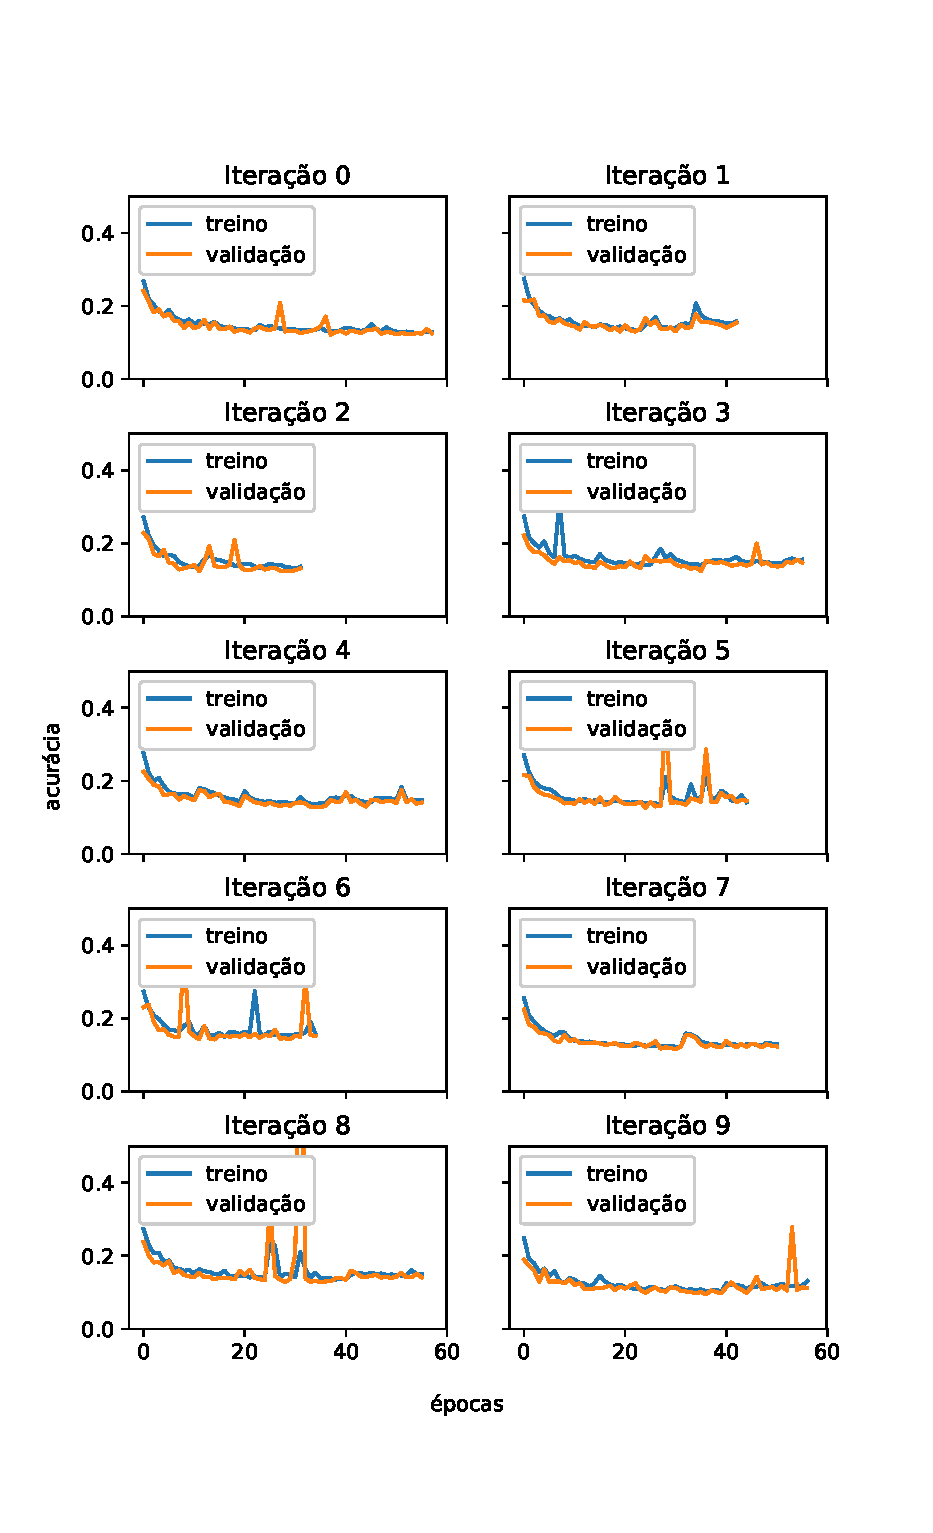
\includegraphics[width=\textwidth, height=\textheight, keepaspectratio]{CapN/1.eps}
\caption{$P_b$; desvanecimentos arbitrários~\mbox{($M=3$).}}
\label{fig:PbmDiversos}
\fonte{a}
\end{figure}


%% Declaração de símbolos, siglas e abreviaturas 
% Pode ser feito em arquivo a parte e incluido com \input
\sigla{DFIG}{Gerador de Indução de Dupla Alimentação}
\sigla{EPS}{{\em Encapsulated Post Script}}
\sigla{PGEEC}{Programa de Pós-Graduação em Engenharia Elétrica e Computação, UNIOESTE, Campus de Foz do Iguaçu (para ocupar 2 linhas)}
\sigla{UNIOESTE}{Universidade Estadual do Oeste do Paraná}


\simbolo{$L$}{Período}
\simbolo{$M$}{Número de ramos de diversidade}
\simbolo{$r_i$}{Envoltória do $i$-ésimo ramo}
\simbolo{$v_c$}{Tensão sobre o capacitor colocado após o retificador para reduzir o {\em ripple} - texto grande para ocupar duas linhas}

\end{document}

